\documentclass[12pt,frame,epsbox]{other/jmyreport}

\usepackage{amsmath}
\usepackage{ltablex}
\usepackage{tabularx}
    \newcolumntype{C}{>{\centering\arraybackslash}X}
    \newcolumntype{L}{>{\raggedright\arraybackslash}X}
    \newcolumntype{R}{>{\raggedleft\arraybackslash}X}

\usepackage{longtable}
\usepackage{type1cm}
\usepackage{colortbl}
\usepackage{multirow}
\usepackage{url}
\usepackage{longtable}
\usepackage{other/a4j}
\usepackage{other/fancybox}
\usepackage{fancyheadings}
\usepackage{other/frame}
%\usepackage{fancyhdr}
\usepackage{other/epsbox}
% 必要な時
%\usepackage{here}
\usepackage[dvipdfmx]{graphicx}
\usepackage[utf8]{inputenc}
\usepackage[dvipdfmx]{hyperref}
\usepackage{pxjahyper}
\begin{document}

%%%%%%%%%%%%%%%%%%%%%%%%%%%%%%%%%%%%%%%%%%%%%%%%%%%%%%%%%%%%
%%% Definitions %%%%%%%%%%%%%%%%%%%%%%%%%%%%%%%%%%%%%%%%%%%%
%%%%%%%%%%%%%%%%%%%%%%%%%%%%%%%%%%%%%%%%%%%%%%%%%%%%%%%%%%%%

\newfont{\mibvii}{cmmib7}
\def\sbmath#1{\mbox{\mibvii #1}}
\def\sbO{\sbmath{O}}
\def\sbo{\sbmath{o}}
\def\sbq{\sbmath{q}}
\def\sbl{\sbmath{l}}
%\def\sbO{\bmath{O}}
%\def\sbo{\bmath{o}}
%\def\sbq{\bmath{q}}
%\def\sbl{\bmath{l}}

\def\lm{m} % 混合における loop 変数
\def\nm{k} % 混合の数

\def\ls{g} % 標本空間の loop 変数
\def\ns{G} % 標本空間の数

\def\sps{\bl} %空間の系列 space sequence
\def\sts{\bq} %状態の系列 state sequence
\def\ssps{\sbl} %空間の系列 space sequence
\def\ssts{\sbq} %状態の系列 state sequence

\def\spsc{l} %空間の系列の要素 space sequence component
\def\stsc{q} %状態の系列の要素 state sequence component

% 太文字フォント
\def\bmath#1{\mbox{\boldmath{$#1$}}}
\def\bA{\bmath{A}}
\def\bB{\bmath{B}}
\def\bC{\bmath{C}}
\def\bD{\bmath{D}}
\def\bE{\bmath{E}}
\def\bF{\bmath{F}}
\def\bG{\bmath{G}}
\def\bH{\bmath{H}}
\def\bI{\bmath{I}}
\def\bJ{\bmath{J}}
\def\bK{\bmath{K}}
\def\bL{\bmath{L}}
\def\bM{\bmath{M}}
\def\bN{\bmath{N}}
\def\bO{\bmath{O}}
\def\bP{\bmath{P}}
\def\bQ{\bmath{Q}}
\def\bR{\bmath{R}}
\def\bS{\bmath{S}}
\def\bT{\bmath{T}}
\def\bU{\bmath{U}}
\def\bV{\bmath{V}}
\def\bW{\bmath{W}}
\def\bX{\bmath{X}}
\def\bY{\bmath{Y}}
\def\bZ{\bmath{Z}}

\def\ba{\bmath{a}}
\def\bb{\bmath{b}}
\def\bc{\bmath{c}}
\def\bd{\bmath{d}}
\def\be{\bmath{e}}
%\def\bf{\bmath{f}}
\def\bg{\bmath{g}}
\def\bh{\bmath{h}}
\def\bi{\bmath{i}}
\def\bj{\bmath{j}}
\def\bk{\bmath{k}}
\def\bl{\bmath{l}}
%\def\bm{\bmath{m}}
\def\bn{\bmath{n}}
\def\bo{\bmath{o}}
\def\bp{\bmath{p}}
\def\bq{\bmath{q}}
\def\br{\bmath{r}}
\def\bs{\bmath{s}}
\def\bt{\bmath{t}}
\def\bu{\bmath{u}}
\def\bv{\bmath{v}}
\def\bw{\bmath{w}}
\def\bx{\bmath{x}}
\def\by{\bmath{y}}
\def\bz{\bmath{z}}

\def\bmu{\bmath{\mu}}
\def\btau{\bmath{\tau}}
\def\bSigma{\bmath{\Sigma}}
\def\bxi{\bmath{\xi}}
\def\bpi{\bmath{\pi}}
\def\btheta{\bmath{\theta}}
\def\bTheta{\bmath{\Theta}}
% 大文字
\def\calC{{\cal C}}
\def\calD{{\cal D}}
\def\calL{{\cal L}}
\def\calN{{\cal N}}
\def\calQ{{\cal Q}}
\def\calS{{\cal S}}

\def\Qfunc{\calQ (\lambda,\overline{\lambda})}
\def\prodt{\displaystyle\mathop{\prod^{T}_{t=1}}}

\def\valueof#1{V(#1)}
\def\spaceof#1{S(#1)}
\def\timeof#1{T({\mbox{\boldmath{$O$}}},#1)}

%
% Σのマクロ

\def\sumt{\displaystyle\sum_{t=1}^{T}} % t=1〜T までの和
\def\sumspace{\sum_{\ls=1}^{\ns}} % 全ての空間に関する和
\def\sumtinspace#1{\displaystyle\sum_{t \in T({\sbO},#1)}}
%\def\sumtinspace#1{\displaystyle\sum_{\textstyle t \in \timeof{#1}}}
% o_t が空間 \ls を含む様な t に関する和

\def\sumonecluster#1{\displaystyle\sum_{c \in \calC(#1)}} % t=1〜T までの和

\newcommand{\bm}[1]{\mbox{\boldmath$#1$}}
\def\argmax{\mathop{\rm argmax}}

\def\tr{\mathop{\rm tr}}
\def\sp{~~~~~}

\newcommand\splittheta[1]{\theta #1^{(1)} + (1-\theta)#1^{(2)}}
\newcommand\diffedsplittheta[1]{\frac{-(#1^{(1)}-#1^{(2)})^2} {(\theta #1^{(1)}+(1-\theta)#1^{(2)})^2}}

%-------------------------------------------------------------
% 表紙
\thisfancypage{}{}
\thispagestyle{empty}

\vspace*{2cm}
\begin{center}
{\Large 2019 年度 \quad 卒業論文}

\vspace{2.5cm}
% \bfseries の後に論文タイトル
%{\Huge \bfseries アルゴリズムを自由に組み替え可能な音声認識デコーダの開発と評価}

%{\Huge \bfseries 仮説生成/選択による大語彙連続音声認識アルゴリズムの統一的表現とそれに基づく汎用デコーダの開発}
{\fontsize{22.5pt}{5pt} \bfseries \mbox{対話状態追跡における}\\} \vspace{0.3cm}
{\fontsize{22.5pt}{5pt} \bfseries \mbox{対話行為タグを用いた重要対話履歴抽出}\\}
\end{center}

\vspace{3.0cm}
\Large
\begin{center}
  \hspace{-4.5cm}{\Large 指導教員}\\
\vspace{0.3cm}
\begin{tabular}{ll}
  {\LARGE 李~晃伸}&{\Large~~教授}\\
  {\LARGE 酒向~慎司}&{\Large~~准教授}\\
\end{tabular}
\end{center}

\vspace{2.0cm}
\begin{center}
名古屋工業大学 工学部\\
情報工学科 \\
{\large 2016 年度入学 ~~~~学籍番号} ~ 28114006 \\
\vspace{1cm}
{\LARGE 石島 \ 侑弥 }\\
\end{center}

% 以下の○○には全体で付けられる通し番号を記入する 修論はない?
\begin{flushright}
  {\LARGE No.37}
\end{flushright}

\normalsize
\newpage

\thisfancypage{}{}
\thispagestyle{empty}

\thisfancypage{}{}
\thispagestyle{empty}

\vspace*{1cm}
\begin{center}
\rule{\textwidth}{.9pt}
\vspace*{2mm}

\uppercase{\large \bfseries BACHELOR DISSERTATION}

\vspace*{1.5cm}

% タイトル
\uppercase{\Large \bfseries Effect of extracting significant dialog history based on dialog act in dialog state tracking}

\vspace*{2cm}

\uppercase{\large \bfseries BACHELOR OF ENGINEERING}

\vspace*{1.5cm}

\uppercase{\large FEBRUARY~~2020}

\vspace*{4mm}

% 氏名.おそらく何をいれても大文字になる
\uppercase{\large \bfseries YUYA~ISHIJIMA}

\vspace*{2.5cm}

% 先生方の名前
{\large
\begin{tabular}{rl}
  Supervisors\,:&
  Professor Akinobu Lee\\
  &Associate Professor Shinji Sako
\end{tabular}
}

\vspace*{1.5cm}

{\large Department of Computer Science\\
  Nagoya Institute of Technology}

\vspace*{2mm}
\rule{\textwidth}{.9pt}
\end{center}
                            % 表紙
%-------------------------------------------------------------
\normalsize
\pagenumbering{roman}
\pagestyle{myheadings}
\setcounter{page}{0}
\tableofcontents                         % 目次
\setlength{\baselineskip}{14.5pt}
\markboth{}{目次}
\listoffigures                           % 図目次
\markboth{}{図目次}
\markboth{}{表目次}
\listoftables                            % 表目次

%-------------------------------------------------------------
\setlength{\baselineskip}{20pt}
\chapter{まえがき}                      % 本文
\pagenumbering{arabic}
\markright{まえがき}
対話システムは,ユーザが持つ要求を対話によって達成することを目的とするタスク指向型対話システムと,対話そのものを目的とする雑談対話システムに大別される.タスク指向型対話システムの例として Apple の「Siri」, NTT の「しゃべってコンシェル」などがあるが,その多くが行う対話は一問一答型である.一問一答型は簡単に実用化できるため多くのシステムで用いられているが,ユーザと応答を繰り返してユーザの細かな要求に対応するという対話はできない.これはシステムが,ユーザが過去の発話で発した要求などといったこれまでの対話の流れを理解していないからである.ゆえに,システムがユーザとの対話の流れを理解するための技術である対話状態追跡(Dialogue State Tracking)が必要とされている.\par
一問一答型ではないタスク指向型対話システムでは,対話状態と呼ばれる対話中のユーザの目的や要求を保持するための枠組みを用いて対話の流れを理解する.対話システムにおける対話状態追跡は,ユーザが発話する度に対話履歴を考慮してその対話状態を維持あるいは更新する役割を担う.そしてシステムは,更新された対話状態を見て次にユーザに対して行う行動や発話を決定することで,ユーザの目的達成に向かった対話を行う.対話状態追跡を行わない場合,システムが過去の対話で得た情報を保持できないのに加え,次の行動を選択できない.そのため,対話状態追跡はタスク指向型対話システムにとって重要な要素である.
\par
現在の対話状態追跡はニューラルネットワークなどの機械学習に基づく手法が盛んに行われている.中でも,深層学習を用いた End-to-End 型のモデル\cite{nbt,e2e}が優れた結果を残しており,発話文から直接対話状態を出力することが可能となった.このようなモデルでは,対話の流れを捉えるために対話履歴を入力に用いる.
\par
対話履歴を全て入力することで対話の流れを捉えられるが,現在の発話との依存関係がない発話が含まれる上に計算量が多くかかる.そのため,従来研究では対話履歴として直近の数発話を入力とする場合が多い.しかし,直近の数発話では対話状態の推定に貢献しない不要な発話が含まれ,必要な発話が含まれない可能性がある.
\par
そこで本研究では,発話者の意図を示す対話行為タグを用いて,対話履歴の中から対話状態の推定に貢献すると思われる発話を抽出する手法を提案する.対話行為タグによって各発話を意図ごとに分類し,特に状態に影響を与える発話を選択的に抜き出すことで,計算量を抑えつつ長い対話履歴を考慮することが可能であると期待できる.
\par
対話システムの国際コンペティションである  Dialog System Technology Challenges 8 Track4 Dialogue State Tracking (DSTC8-Track4)\cite{dstc8} において,対話状態追跡のデータセットとベースラインモデルが公開されている.本研究では DSTC8-Track4 のデータセットとモデルを用いて実験を行い従来法との比較を行う.\par
以下,第 2 章では近年の対話システムにおける対話状態追跡とその問題点について,第 3 章では本研究におけるベースラインモデルについて述べる.また,第 4 章では提案手法について述べる.
第 5 章ではどの対話行為タグを持つ発話が重要なのかを調査した予備実験の結果を示し,第 6 章では提案手法の結果と分析,さらに従来手法との比較を示す.第 7 章では,むすびと今後の課題について述べる.

%-------------------------------------------------------------
\chapter{対話システムにおける対話状態追跡}
%対話状態追跡はなんなのか
本章ではタスク指向型対話システムと対話状態追跡の説明をした後,これまでの対話システムがどのような手法によって対話状態追跡を行ってきたか,また何が問題であったかを順に説明する.そして,本研究が取り扱ったコンペティション DSTC8-Track4 について説明する.
\markright{対話システムにおける対話状態追跡}
\section{タスク指向型対話システム}
ユーザとシステムが行う対話は大きく分けると,タスク指向型対話と雑談対話の 2 種類が存在する.タスク指向型対話とは,ユーザが特定の目的を持ち,ユーザとシステムが応答を繰り返すことでその目的を達成する対話のことである.雑談対話とは,対話そのものを目的として行うもので,明確な目的が存在しない対話のことである.また,前章で述べた一問一答型の対話はタスク指向型対話の一部で,対話状態を用いずに一回の応答でユーザの要求に応える対話のことである.一問一答型の対話は一回の応答で対話が完結するため,ユーザの細かい要求に応えられないという問題がある.
\par
タスク指向型対話システムとは,タスク指向型対話を行う対話システムのことであり,ホテル案内,レストラン案内,交通案内など様々なドメインを扱う.タスク指向型対話システムの実用例として,バス案内システムとして実運用されている「Let's Go システム」\cite{letsgo} や大学のキャンパス案内を行う「正門メイちゃん」\cite{mmdagent}が挙げられる.
\par
\begin{figure}[thb]
  \centering
  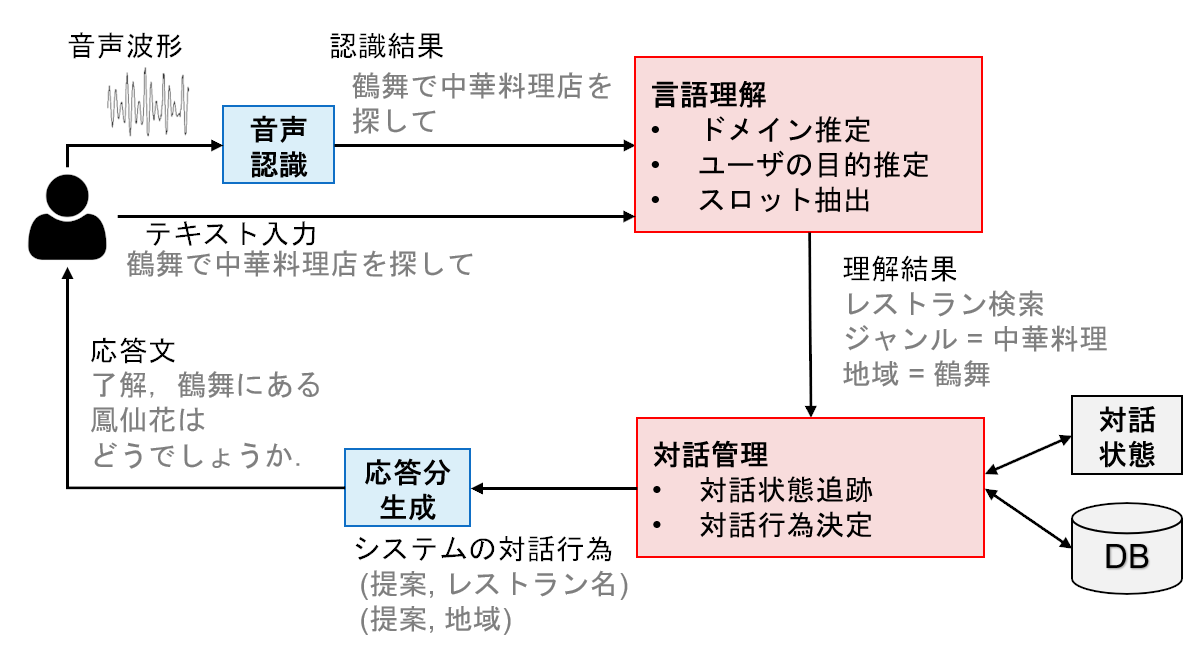
\includegraphics[width=15cm]{chapter2/system3.eps}
  \caption{タスク指向型対話システムの基本構成}
  \label{fig:taiwasystem}
\end{figure}
タスク指向型対話システムの基本構成を図\ref{fig:taiwasystem}に示す.対話システムは大きく分けて,音声認識部,言語理解部,対話管理部,応答生成部の4つのモジュールで構成されている.音声認識部はユーザの発話音声を認識し発話文に変換し,言語理解部はその発話文をシステムが理解できる形に変換する部位である.言語理解部が行うことは,発話文からユーザが行おうとしているタスクのドメインが何か推定するドメイン推定,そのドメイン中でのユーザの目的は何か推定するユーザの目的推定,発話中に含まれるスロットの値候補を見つけるスロット抽出の 3 つである.スロットとはドメインごとに与えられる属性のことで,システムはスロットと値の組によってユーザの要求を表現する.そして対話管理部は,過去の発話も考慮してユーザの目的と要求を推定する対話状態追跡と,対話状態から不足している情報を検出し次のシステムの行動を決定する対話行為決定を行う.最後に,応答文生成部でシステムの対話行為に沿った応答文を生成する.このようにタスク指向型対話システムは,4つのモジュールでユーザとのタスク指向型対話を可能にする.

\section{対話状態追跡}
\begin{figure}[tbh]
    \centering
    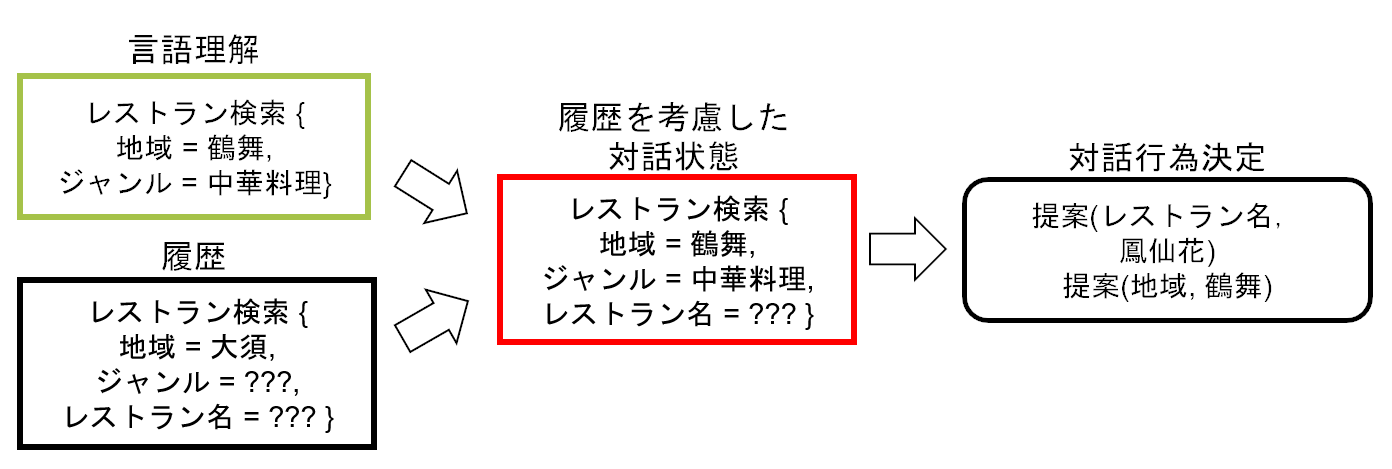
\includegraphics[width=15cm]{chapter2/dst2.eps}
    \caption{対話管理部の処理の流れ}
    \label{fig:dst}
\end{figure}

対話システムにおける対話状態追跡は,図\ref{fig:taiwasystem}に示した通り対話管理部の機能の1つである.対話管理部の処理は図\ref{fig:dst}のような流れになっている.対話状態追跡は言語理解の結果と履歴を考慮して,対話状態を出力する.この図において,履歴は一例として前のターンの対話状態を用いている.対話状態はレストラン検索などといった目的と,スロットと値の組を用いた辞書形式で表現される.システムは対話状態にある目的を達成するために必要なスロットを埋めていく作業を行う.つまり,対話状態追跡は対話状態のスロット値を言語理解の結果から得たスロット値候補に変更するか否かを判断する役割を担う.また,対話行為決定では対話状態の不足している情報を検出して,目的達成に向けて必要なシステムの対話行為を選択する.
\par
システムは対話状態を見て次の行動を決めるため,対話状態追跡が対話状態の推定を誤ると,ユーザの要求にそぐわない対話を行うことになる.ゆえに対話状態追跡はタスク指向型対話システムにとって重要な要素である.

\section{ルールベースの対話状態追跡}
\begin{figure}[thb]
  \centering
  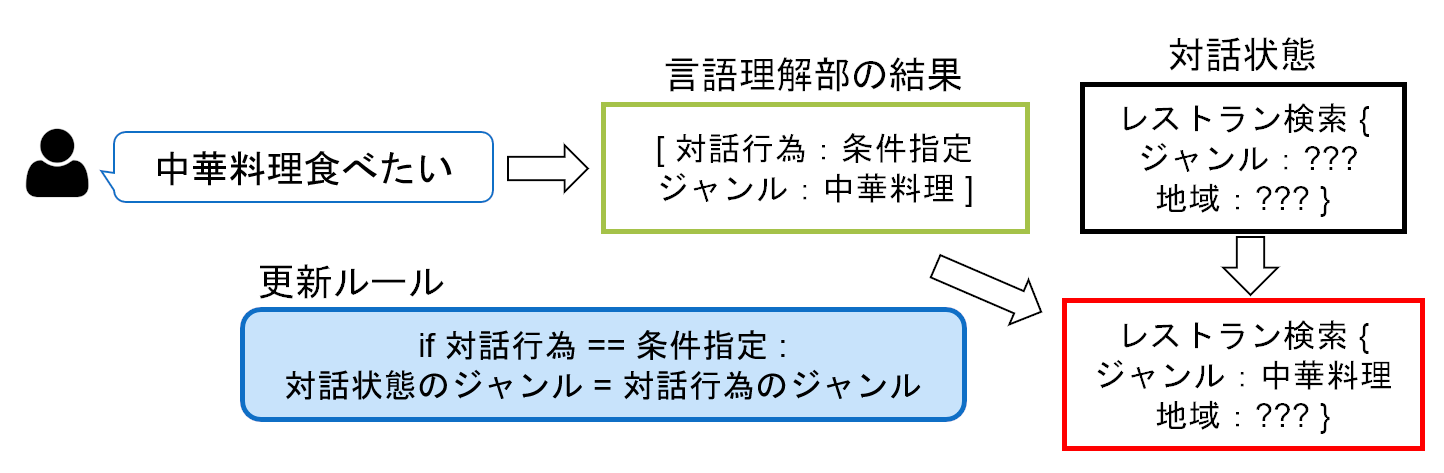
\includegraphics[width=15cm]{chapter2/rulebase.eps}
  \caption{if-then ルールによる対話状態追跡の例}
  \label{fig:rulebase}
\end{figure}

ルールベースの対話状態追跡とは,予め人間が決めた規則に従って対話状態を更新する対話状態追跡のことである.その規則は更新ルールと呼ばれ,プログラムやグラフによって定められる.
\par
一例として,if-then 文で記述されたプログラムを用いた対話状態追跡を図\ref{fig:rulebase}に示す.ルールベースの対話システムは図\ref{fig:rulebase}のように,言語理解部でユーザの対話行為も推定する.そして対話状態追跡は,言語理解部から得たユーザの対話行為によって条件分岐を行い,対話状態を更新していく.
\par
ルールベースの対話状態追跡は,後述する統計的機械学習や深層学習による対話状態追跡に比べて容易に行えるため,ほとんどの商用対話システムで採用されている.ただし,複雑な対話を扱うには多くの規則を定義する必要がある.また,言語理解部の結果に大きく依存するため,言語理解部で誤りが発生すると,自ずと間違った情報が対話状態に追加されるという問題がある\cite{rule_base}.
\section{統計的機械学習による対話状態追跡}
\begin{figure}[thb]
  \begin{center}
    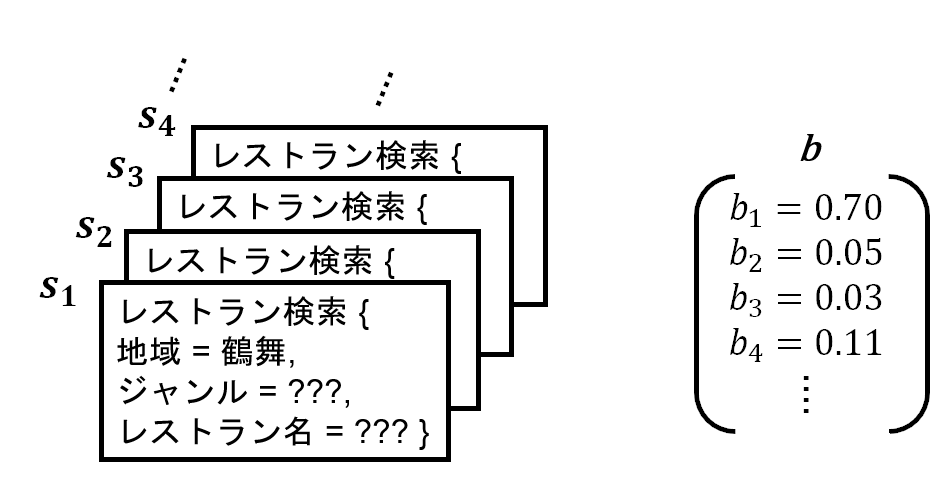
\includegraphics[width=10cm]{chapter2/belief.eps}
    \caption{対話状態の確率的表現である信念$b$ のイメージ図}
    \label{fig:belief}
  \end{center}
\end{figure}

統計的機械学習による対話状態追跡では,言語理解部からの誤りに対する頑健性を得るために,対話状態を確率的に扱う.これは,ユーザ発話の解釈に不確実性が存在するため,対話状態を直接観測できないとしているからである.対話状態の確率的表現は,全ての対話状態にわたる確率分布である信念 $b$ を用いる.信念に関する図を図\ref{fig:belief}に示す.また,言語理解部の出力はノイズを含むユーザ入力の観測 $o$ とし,対話状態の集合を$I_s$,システムの行動の集合を$K$とする.対話状態の推定は,ターン $t$ の対話状態を $s^t \in I_s$,
システムの対話行為を $a^t \in K$,観測状態を $o^t \in I_s$,ユーザの対話状態が$s$である信念(確率変数)を $b^t_s$ として,式\ref{joutai_suitei}を推定する問題となる.
\begin{equation}
  \label{joutai_suitei}
  b_s = P(s|o^{1:t})
\end{equation}
$P(s|o^{1:t})$ は,これまでの観測状態から推定した全てのユーザの対話状態にわたる確率分布である.つまり,履歴としてこれまでの観測状態を用いている.
\par
統計的機械学習による対話管理の一例として,部分観測マルコフ決定過程(Partially Observable Markov Decision Process ; POMDP)\cite{pomdp,pomdp_review}を用いた手法を説明する.POMDPベースのモデルは,信念状態の追跡と強化学習という2つのキーアイデアを組み合わせている\cite{pomdp_review}.
強化学習とは,システムの行動に対して報酬を与えることで,システムに報酬を最大化する行動を学習させるという機械学習の一種である.
\par

\begin{figure}[thb]
  \begin{center}
    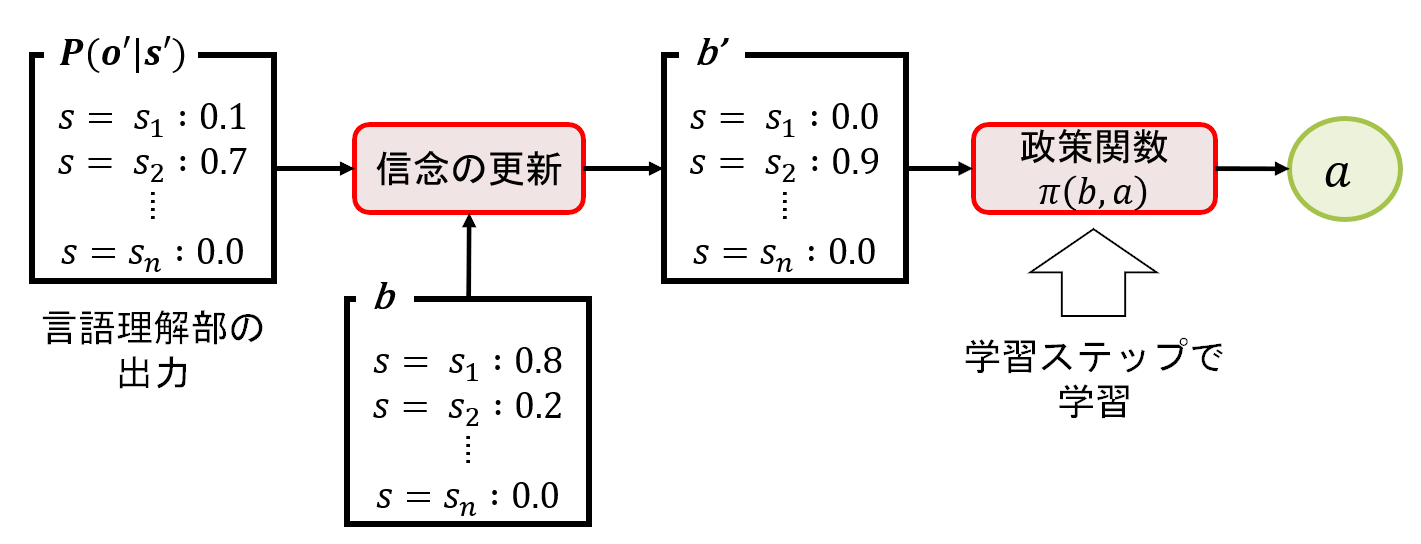
\includegraphics[width=15cm]{chapter2/pomdp2.eps}
    \caption{部分観測マルコフ決定過程(POMDP)の流れ}
    \label{fig:pomdp}
  \end{center}
\end{figure}


POMDPを用いた対話管理は図\ref{fig:pomdp}のように,言語理解部の出力を全ての対話状態にわたる確率分布 $p(o'|s')$ で表す.そして,信念状態の追跡には対話状態を最新の対話状態に更新する状態更新関数を用いる.状態更新関数は現在の対話状態 $s^{t+1}$ をこれまでの観測状態系列 $o^{1:t+1}$ から求める式である.状態更新関数は式\ref{state_update}に示す.
\begin{equation}
  \label{state_update}
  b' = P\left(s^{t+1}|o^{1:t+1}\right) \propto P\left(o'|s'_{j}\right) \Sigma_{s_i} P\left(s'_{j}|s_i, \widehat{a_k}\right)b^t
\end{equation}
式\ref{state_update} では,$P(o'|s'_j)$が観測確率,$P(s'_j|s_i,\widehat{a_k})$ が状態遷移確率,$b_t$が現在の信念を表す.
信念の更新をした後,状態 $s$ で対話行為 $a$ を選ぶ確率である政策関数$\pi (b,a)$を用いて次のシステムの対話行為を決める.POMDP での報酬は状態行動価値(Q値)などを用いる.Q 値とは,ある状態$s$のとき対話行為$a$を行い得られる報酬の期待値である.POMDPを用いた対話管理は,その報酬を用いて政策関数を強化学習により最適化していき,最適なシステムの対話行為を選ぶことを目指す.
\par
POMDPを用いた対話管理は,全ての状態にわたる信念の分布を維持することにより,システムは全ての可能な対話経路を効果的に並行して追求し,最も可能性の高い状態だけではなく,全ての状態にわたる確率分布に基づいて次の対話行為を選択することが可能になる\cite{pomdp_review}.
問題としては,複雑な対話を取り扱うと対話状態のパターンが増加するため,信念の追跡が困難になることがある.また,ルールベースほどではないが言語理解部の誤りにより性能が悪化する.
\section{深層学習による対話状態追跡}
深層学習は,人間の神経細胞の仕組みを模したシステムであるニューラルネットワークがベースになっている\cite{deeplearning}.そして,ニューラルネットワークを多層にして用いることで,データに含まれる特徴を段階的により深く学習することが可能になる.深層学習を行う場合,ラベル付けされたデータが必要になるが,現在はDSTC2\cite{dstc2}やMulti-Woz\cite{multi-woz}など,ユーザの対話状態やシステムの対話行為などをラベル付けした対話データセットが公開されている.このようなデータが公開されたことで,深層学習による対話状態追跡の研究が盛んに行われている.
\par
深層学習による対話状態追跡では,通常発話文を入力として直接対話状態を出力する\cite{nbt,e2e}.対話状態であるインテントや各スロットの値に関してはデータセットによって事前に候補が与えられている.そのため,発話文から得た情報を基にそれぞれの全候補にわたる確率分布を出力し,確率最大のものをインテントあるいはスロット値として選択する.しかし,そのようなモデルは候補として与えられていない値を推測できないため,言語理解などを用いて候補外の値も推定可能にするモデル\cite{joint,trade,mrc}の研究が行われている.そのようなモデルの例として,Rastogi ら\cite{joint} のモデルを図\ref{fig:joint}に示して説明する.
\begin{figure}[t]
  \begin{center}
    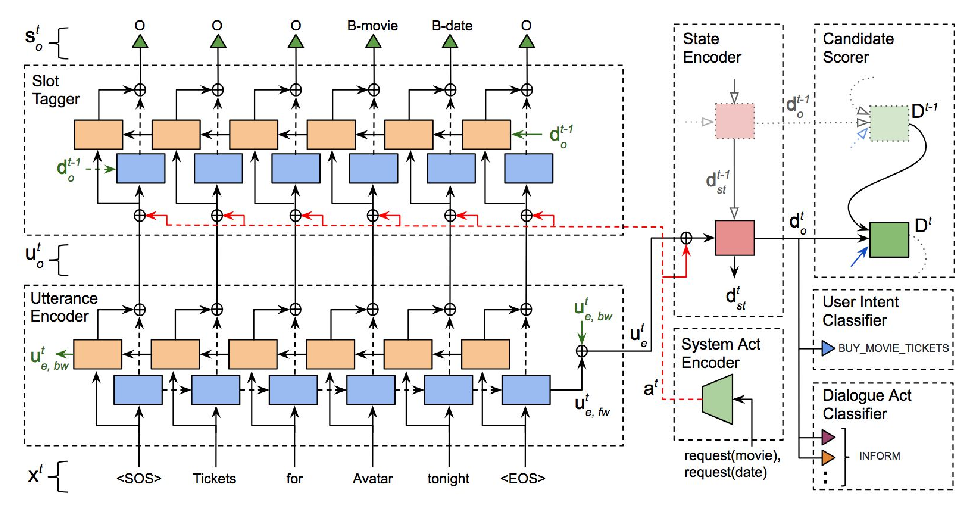
\includegraphics[width=15cm]{chapter2/joint.eps}
    \caption{言語理解と対話状態追跡を共同で学習するモデル\cite{joint}}
    \label{fig:joint}
  \end{center}
\end{figure}
このモデルは,Utterance Encoder, System Act Encoder, State Encoder によってユーザの発話,システムの対話行為,対話状態の特徴量を得る.これら特徴量は言語理解部と対話状態追跡部で共有される.言語理解部である Slot Tagger は発話中の単語ごとにラベルを付けてスロット値の候補となる単語を見つける.ラベルは,スロット値の開始地点を示す B ラベル,スロット値の継続を示す I ラベル,スロット値でないことを示す O ラベルで構成される IOB ラベルが用いられる.B ラベルと I ラベルはスロットの数だけ作成される.Slot Tagger で見つけられたスロット値はスロット値候補リストに追加される.対話状態追跡部は,User Intent Classifierでユーザの目的を推定し,Dialogue Act Classifierでユーザの対話行為を推定し,Candidate Scorer でスロット値候補リスト中の候補のランク付けを行いスロットに値を割り当てる.
\par
言語理解と対話状態追跡を共同で学習することで,言語理解部で発生した誤りが対話状態追跡部に伝搬するのを防ぐことが可能になる.また,言語理解部と対話状態追跡部でエンコーダのネットワーク層を共有できるため,性能の向上とネットワーク層のパラメータの数の削減が同時に行える\cite{joint}.しかし,このようなモデルは新しいドメインに適応させたい場合,言語理解部のIOBラベルを増やして再学習する必要がある.したがって,現在は新しいドメインに再学習なしで適応可能な拡張性のある対話状態追跡の研究が注目されている.
\section{Dialogue System Technology Challenge 8}
%こういうコンペがあります
Dialog System Technology Challenges 8 (DSTC8) \cite{dstc8}とは対話に関するコンペティションである.2013 年に最初の Dialog State Tracking Challenge(対話状態追跡タスク)が開催された.第 6 回から対話状態追跡だけでなく,対話破綻検出や応答生成といった対象となるタスクの幅が広がり,略称はDSTCのままで現在の Dialog System Technology Challenges へと名称が変更された.
\par
ここでは本研究で取り組んだ対話状態追跡タスクの DSTC8-Track4 について説明する.昨今,ホテル案内や交通案内などのドメインを行えるサービスが多く存在している.サービスごとに様々な バックエンドAPI が定義されるため,同じドメインでもシステムが理解できず,対応させるには再学習が必要となる.
DSTC8-Track4では,現在の対話システムの課題の1つである新サービスへの拡張を再学習なしで可能にすることを目的としており,そのための対話状態追跡モデルを作成する.
\par
本タスクでは,ユーザが対話で達成したい目的をインテントと呼ぶ.インテントはサービスごとにいくつか存在する.例えばレストランサービスであれば,レストラン検索(FindRestaurant)とレストラン予約(ReserveRestaurant)が存在する.システムはサービスに対応するインテントの変化を追跡することで,ユーザの目的に合った質問や返答を返すことが可能になる.
\par
また,本タスクではサービスを定義する枠組みであるスキーマが用意されている.スキーマは,サービスごとにスロットのリストとインテントのリストを持つ.スキーマの構成は図\ref{fig:schema}に示す.
\begin{figure}[thb]
    \centering
    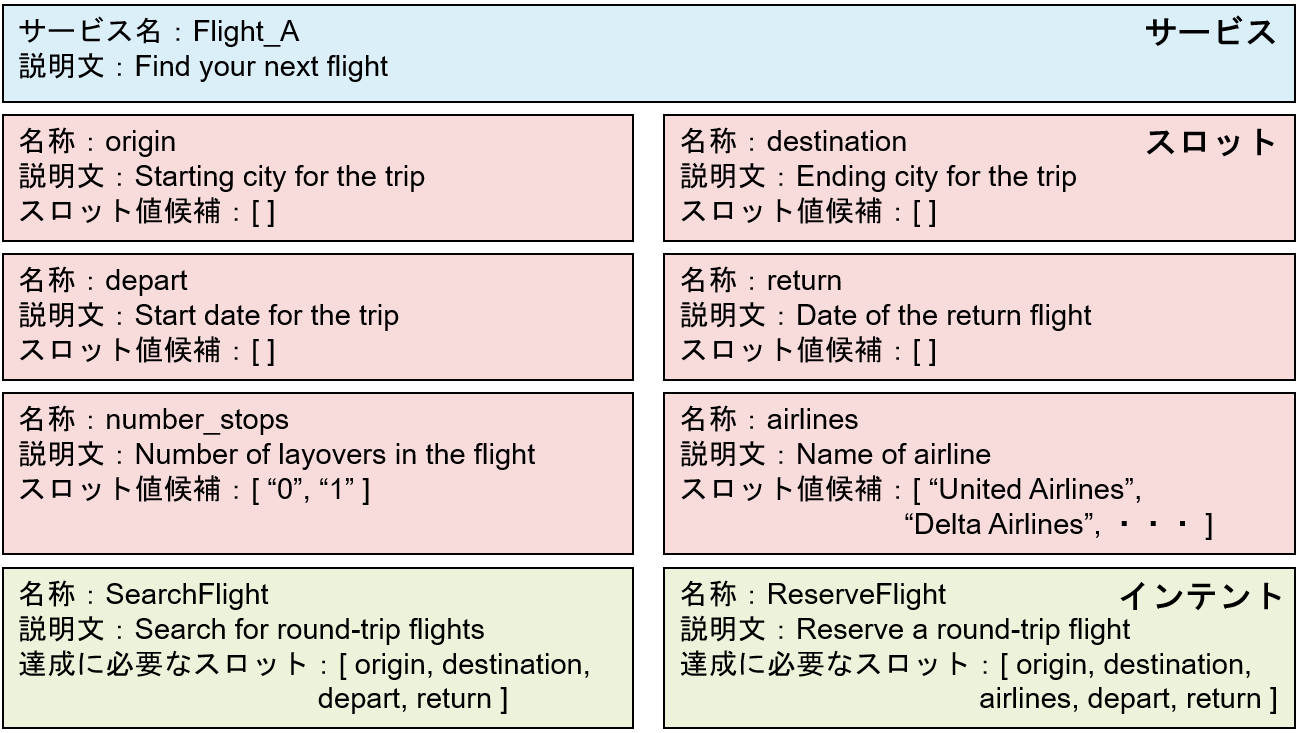
\includegraphics[width=15cm]{chapter2/schema2.eps}
    \caption{スキーマの構成}
    \label{fig:schema}
\end{figure}
スキーマには,サービス,スロット,インテント全てに説明文が付与されている.この説明文によって,システムが未知のサービス,スロット,インテントを理解することを可能にする.スロットに関してはスロット値候補を持つ候補ありスロットと,候補を持たない候補なしスロットに分けられる.候補ありスロットはスロット値を事前に与えられている候補から選択するが,候補なしスロットはスロット値を発話文中から抜き出す必要がある.図\ref{fig:schema}では,乗り換えの回数を表す“number\_stops”スロット,航空会社を表す“airlines”が候補ありスロット,出発地を表す“origin”スロット,到着地を表す“destination”スロットなどそれ以外が候補なしスロットにあたる.また,各インテントの達成に必要なスロットという情報を持つため,システムはスキーマによってサービスの バックエンドAPI が何を必要としているかを理解できる.
\par
\begin{figure}[t]
    \centering
    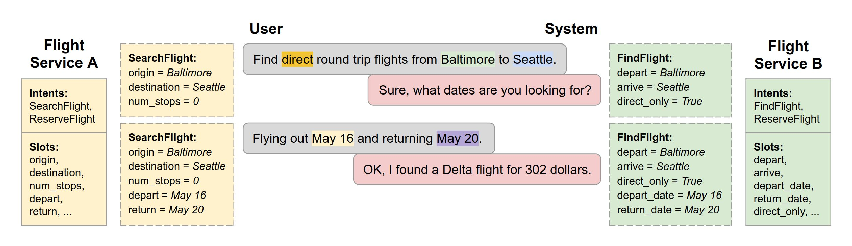
\includegraphics[width=15cm]{chapter2/dstc8-track4.eps}
    \caption{DSTC8-Track4 のイメージ図\cite{dstc8}}
    \label{fig:dstc8-track4}
\end{figure}
本タスクは,学習時,検証時,テスト時それぞれで扱うサービスが異なる.図\ref{fig:dstc8-track4}に示した通り,同じ “Flight Service” でもインテントの候補とスロットが異なる名前で定義されている.そして,どちらのサービスを扱うとしても,ユーザの目的と要求を同様に推定できる対話状態追跡モデルを作成する必要がある.
\par 
参加者はベースラインモデルと整形された対話データセットが配布され,そのデータセットなどを用いて作成したモデルの学習と評価を行い,モデルと評価結果を提出する.
\par 
配布されたデータセットは SGD データセットと呼ばれ,人とシステムの間のラベル付きタスク指向型対話を持つ.各対話はユーザとシステムが交互に 1 発話ずつ行い,1 発話につき 1 ターンとしている.1 ターンごとに,発話中に存在するスロット値候補の位置を範囲で示すスロット値範囲リストが与えられる.スロット値範囲リストは以下の要素を持つ.
\begin{itemize}
    \item スロット - スロットの名前
    \item 開始位置 - 発話中にあるスロット値候補の開始位置
    \item 終了位置 - 発話中にあるスロット値候補の終了位置
\end{itemize}
対話状態はユーザのターンのみ与えられる.対話状態は以下の要素を持つ.
\begin{itemize}
    \item インテント(Noneを含む)
    \item 要求スロット - ユーザが値を要求しているスロットのリスト
    \item スロット値 - 各スロットに当てはまる値
\end{itemize}
対話状態の推定は,この3つの要素を全て推定する必要がある.
また,対話行為はシステムのターンのみ与えられる.本タスクの対話行為は,システムがあるスロットに対してどのような行動をしたのかを示すため,以下の要素を持つ.
\begin{itemize}
    \item 対話行為タグ - 対話行為の種類を示す
    \item スロット - 対話行為が関与しているスロット
    \item スロット値 - 対話行為で用いたスロット値
\end{itemize}
例えば “OFFER (origin, Baltimore)” ならば,出発地として “Baltimore” を提案するという行動を示す.
\par
本タスクでは,発話文,スキーマ,対話行為を入力として,対話状態であるインテント,要求スロット,スロット値を推定する.スロット値に関して,候補ありスロットではスロット値をスキーマから与えられるスロット値候補から推定し,候補なしスロットではスロット値となる文字列の範囲を発話中から推定する.候補なしスロットの推定では,既にスロットに割り当てられている値と同じ意味の値(例:“at afternoon 1:30”, “1:30 pm”)を推定することがあるため,候補なしスロットには複数の値が割り当てられることもある.
%-------------------------------------------------------------
\chapter{BERTに基づく対話状態追跡}
\markright{BERTに基づく対話状態追跡}
本研究で提案する手法を試すために,DSTC8 Track4 で公開されたベースラインモデル\cite{baseline}を用いた.本章では,ベースラインモデルとして用いた BERT に基づく対話状態追跡について述べる.
\section{BERT とは}
BERT(Bidirectional Encoder Representations from Transformers)とは,Google が2018年に発表した自然言語処理モデルである\cite{bert}.Recurent Neural Network などを使わずに Attention機構のみを用いた Transformer \cite{transformer} と呼ばれるモデルがある.Transformer が 文脈を単一方向しか考慮しないのに対して,双方向考慮するように改良したのが BERT である.BERT の特徴として,事前学習モデルであることが挙げられる.従来のニューラルネットワークを用いた自然言語処理モデルは,言語理解や感情推定など特定のタスクのみに対応しており,タスクに応じた出力を行う.しかし,事前学習モデルである BERT は既存のタスク実行モデルに付け加えるだけで,そのモデルの性能を向上させることが可能である.
\par
BERT を付け加える際には,入出力をタスクに合わせたものに置き換えて追加学習する Fine-Tuning という手法が用いられる.そのようなモデルの中での BERT は,入力文の埋め込み表現を得るために用いられる.自然言語処理における埋め込みとは,文や単語,文字など自然言語の構成要素に対して,何らかの空間におけるベクトルを与えることであり,ベクトルには文や単語の特徴量が格納される.図\ref{fig:bert_fine}のように,BERTは2つの文章を入力として,単語単位に分割する.分割したものをトークンと呼ぶ.また,入力した文の初めに“[CLS]”,2つの文章の末尾に“[SEP]”という特殊なトークンを挿入する.そして,BERTは文章ペア全体の埋め込み表現とトークンレベルの埋め込み表現を抽出する.BERTに付け加えたタスク実行モデルは,これら埋め込み表現を用いて各タスクに合わせた出力を学習していく.また,BERT 自体もタスクに合うように埋め込み表現を更新していく.
\par
  
\begin{figure}[tbh]
  \centering
  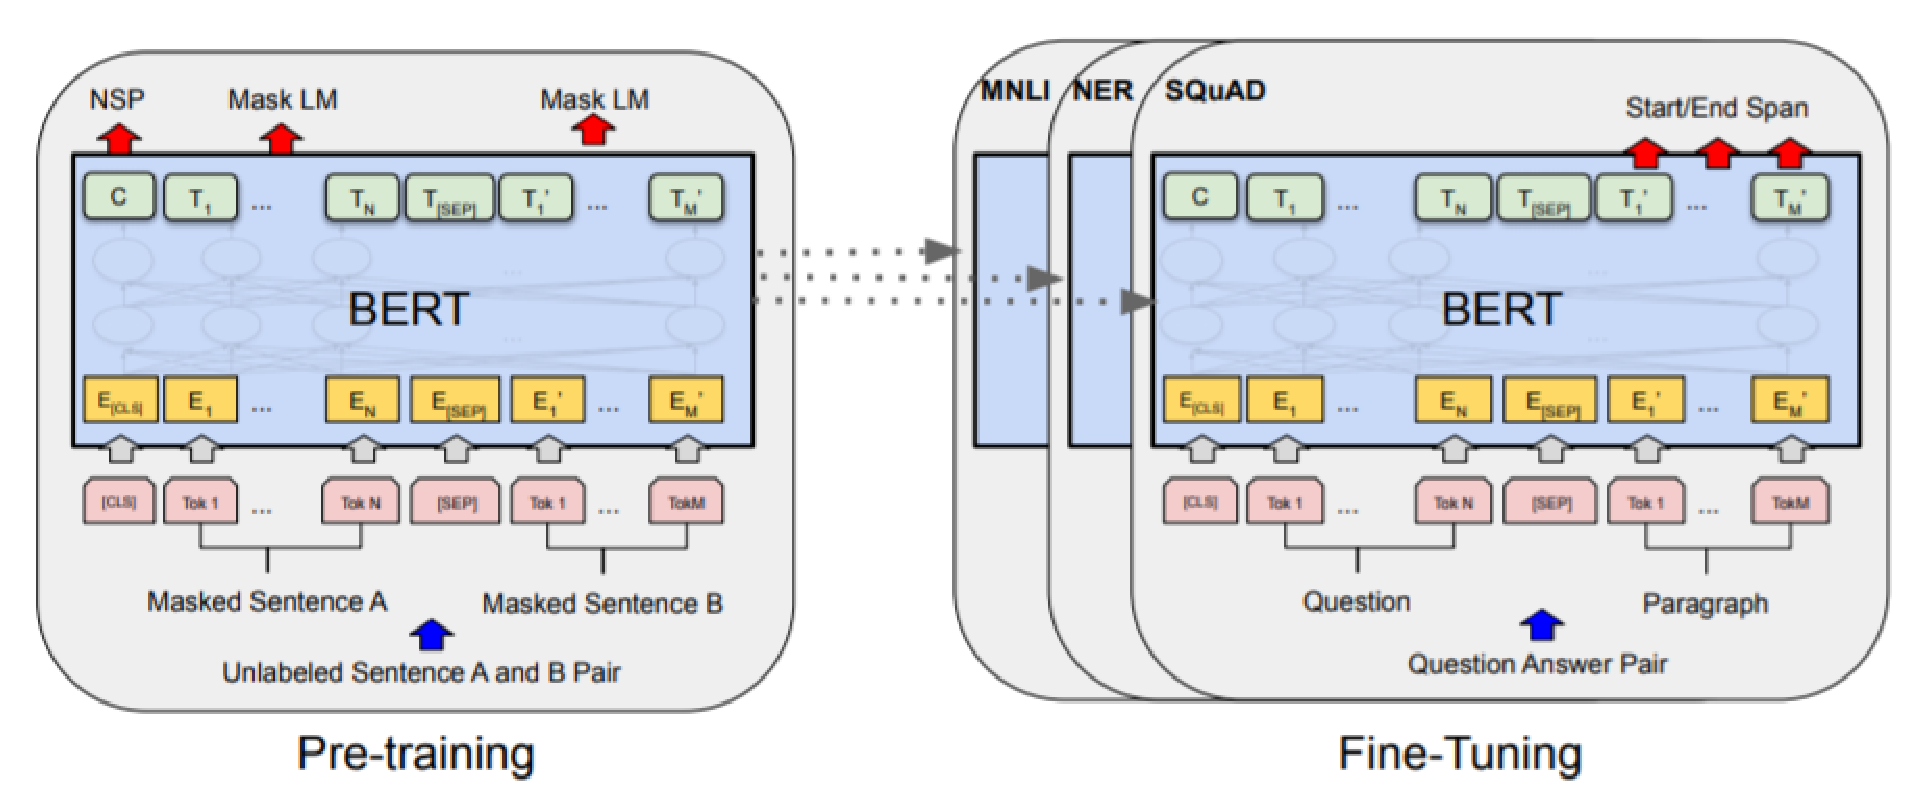
\includegraphics[width=15cm]{chapter3/bert_fine.eps}
  \caption{Fine-Tuningの例\cite{bert}}
  \label{fig:bert_fine}
\end{figure}

BERT は汎用性の高さが評価され注目を浴びている.加えて,少ないデータで追加学習を行うだけで動作するため,自然言語処理分野の長年の課題であったデータ不足を解決する.自然言語処理分野でデータが不足していた原因は,データ収集やラベルの付与に多大なコストと時間がかかることが挙げられる.しかし,BERT の事前学習では Wikipedia や BooksCorpus などから得た大量のラベル未付与のデータを用いて,前後の文脈を加味したトークンの埋め込み表現や2つの文章の関係性を事前に学習する.そのため,少量のラベル付きデータで追加学習を行うだけでタスクの実行が可能になる.ゆえに,本研究でも BERT による対話状態追跡モデルをベースラインとして用いる.
\section{BERTに基づく対話状態追跡}
\begin{figure}[thb]
    \centering
    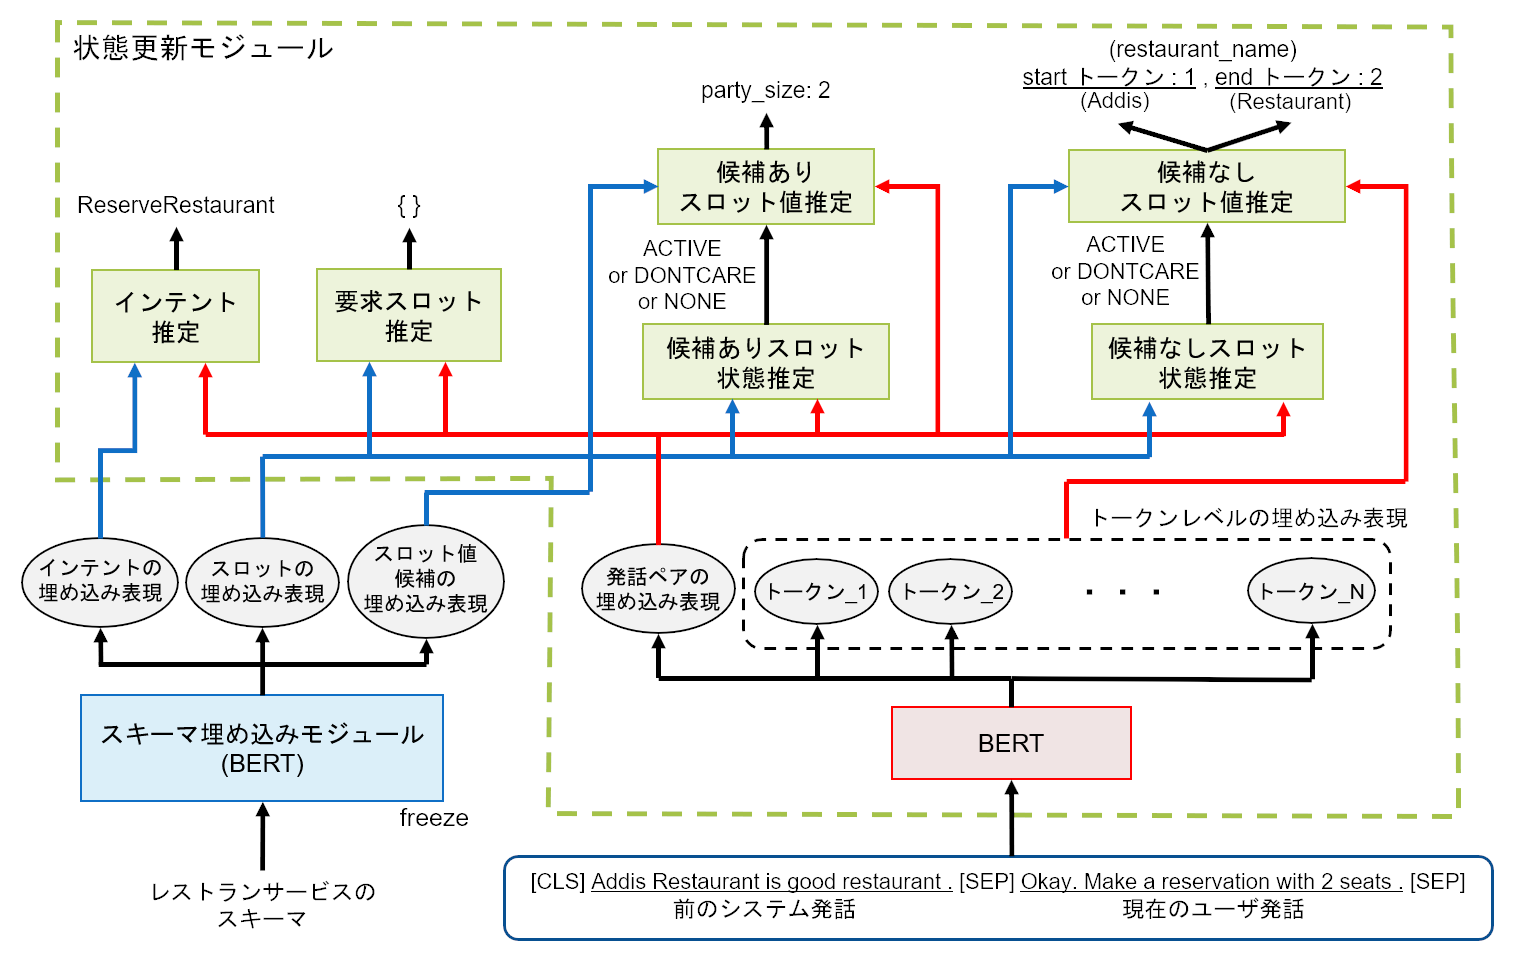
\includegraphics[width=15cm]{chapter3/baseline.eps}
    \caption{ベースラインモデルの構成}
    \label{fig:baseline}
  \end{figure}

本トラックで提供されたベースラインモデルは,BERT を用いた Fine-Tuning で対話状態追跡を行うモデルである.ベースラインモデルは図\ref{fig:baseline} のように,スキーマ埋め込みモジュールと状態更新モジュールの2種類のモジュールで構成されている.
\subsection{スキーマ埋め込みモジュール}
スキーマ埋め込みモジュールは,図\ref{fig:baseline}のように,BERT を用いてスキーマに含まれているインテント,スロット,スロット値候補の埋め込み表現を抽出する.インテントは,\{[CLS] [サービスの説明] [SEP] [インテントの名称] [インテントの説明] [SEP]\} をBERTへの入力として,埋め込み表現を抽出する.スロットは,\{[CLS] [サービスの説明] [SEP] [スロットの名称] [スロットの説明] [SEP]\} で入力し,埋め込み表現を得る.ただし,要求スロットの推定に用いる全てのスロットの埋め込み表現,候補ありスロットの状態推定に用いる候補ありスロットの埋め込み表現,候補なしスロットに関する推定に用いる候補なしスロットの埋め込み表現という3種類を抽出する.スロット値候補は,\{[CLS] [候補ありスロットの名称] [候補ありスロットの説明] [SEP] [スロット値候補] [SEP]\} をBERTへの入力として,埋め込み表現を抽出する.
\par
スキーマ埋め込みモジュールで用いる BERT は事前学習されているものを用いるため,出力される埋め込み表現は事前に計算されたもので,学習によって更新されることはない.
\subsection{状態更新モジュール}
状態更新モジュールの学習に用いるサンプルは各ユーザターンごとに生成される.各サンプルには,入力文となる現在のターンのユーザ発話,前のターンのシステム発話に加えて,扱うサービスのスキーマ埋め込み表現,各種正解ラベルが含まれる.状態更新モジュールはそのサンプルを用いて,インテント,要求スロット,スロット値を推定するように学習する.なお,このモジュールでは発話にまたがるスロット値の維持は行っていないため,推定できるスロット値は入力文中に含まれる値のみである.
\par
まず初めに状態更新モジュールは各サンプルのユーザ発話と前のシステム発話が BERT に送られ,BERT は発話ペアの埋め込み表現とトークンレベルの埋め込み表現を出力する.その後,インテント推定,要求スロット推定,スロット値推定を共同で学習する.モデルは直近の発話 2 つを入力として使用するため,前のユーザターンからの対話状態の差異を推定するように学習する.そのため,スロット値の推定はスロットが更新されるか否かを出力するスロット状態推定と更新されると判断されたスロットの値を推定するスロット値推定の2段階で行われる.また,スロット値の推定は候補ありスロットと候補なしスロットに分けて行われるため,状態更新モジュールは合計で 7 つの推定を共同で学習する.
\par
\begin{itemize}
    \item
    インテント推定は,現在のターンにおけるインテントを推定する.インテント推定では,まず初めに,発話ペアの埋め込み表現とスキーマの埋め込みに含まれる各インテントの埋め込み表現を連結する.各インテントの埋め込みには,インテント無しを表す NONE インテントの埋め込み表現も含まれる.連結された埋め込み表現は訓練可能な射影を使用してロジット値に射影される.ロジット値(logit)とは,確率 $p$ で起こる事象 A について,A が起こる確率と起こらない確率の比の対数 $\log(p / (1-p))$ である.得られた全てのインテントのロジット値は Softmax 関数で正規化され,サービス中の全てのインテントにわたる確率分布が生成される.そして,確率が最大のインテントがそのターンにおけるインテントであると推定される.
    \item
    要求スロット推定は,ユーザがスロット値を要求しているスロットを推定する.要求スロット推定では,発話ペアの埋め込み表現と全てのスロット埋め込みを用いて,インテント推定と同様の方法でロジット値を取得する.そして,各ロジット値は Sigmoid 関数を使用して正規化され,その値を各スロットのスコアとする.スロットのスコアが 0.5 を超える場合,そのスロットは要求スロットであると推定される.
    \item
    スロットの状態として,NONE, DONTCARE, ACTIVE を定義する.NONEはスロット値が変更されないことを示し,DONTCAREはユーザがそのスロットに対して関心がないことを示し,ACTIVEはスロット値が更新されることを示す.スロット状態推定では各スロットに対してどの状態であるかを推定する.入力は,候補ありスロット状態推定ならば候補ありスロットの埋め込み表現,候補なしスロット状態推定ならば候補なしスロットの埋め込み表現を発話ペアの埋め込み表現と連結する.連結した埋め込み表現から,訓練可能な射影を使用して,NONE, DONTCARE, ACTIVEのロジット値を取る分布を取得する.スロットの状態が NONE と推定された場合,スロット値が変更されない.DONTCAREと推測された場合,スロット値として dontcare が割り当てられ,ACTIVE と推測された場合,次に行われるスロット値推定でスロット値が推定される.
    \item
    候補ありスロット値推定は候補ありスロットに割り当てられる値を推定する.候補ありスロット推定では,発話ペアの埋め込み表現とスロット値候補の埋め込み表現を連結して,インテント推測と同様の方法で各スロット値候補のロジット値を得る.得られた全てのロジット値は,Softmax 関数を使用して正規化され,スロット値候補の確率分布が生成される.そして,確率が最大である値がスロットに割り当てられる.
    \item
    候補なしスロット値推定は,入力文中の単語からスロット値となる文字列を抜き出す必要があるため,スロット値となる文字列の範囲を推定するように学習する.範囲の推定では,BERT モデルから取得したトークンレベルの埋め込み表現と候補なしスロットの埋め込み表現を連結する.そして,連結した埋め込み表現は訓練可能な射影を使用してロジット値に変換される.得られた全てのトークンのロジット値は,Softmax 関数を使用して正規化され,全てのトークンにわたる確率分布にされる.この分布は,範囲の開始位置である start を推定するように学習する.また,異なる重みセットを使用した同様の手順で,範囲の終了位置である end の分布も推定する.推論中,start と end の確率の和が最大になるトークンの組み合わせが推定され,その範囲にある文字列がスロットに割り当てられる.
\end{itemize}
\par
これら7つの推定では,それぞれで交差エントロピー誤差を計算する.計算した7つの誤差の和をこのモデルの誤差として学習に用いる.
%-------------------------------------------------------------
\chapter{対話行為タグを用いた重要対話履歴抽出}
\markright{対話行為タグを用いた重要対話履歴抽出}
本章では,SGD データセットに含まれる対話行為タグの種類を説明したのち,本研究で提案する対話行為タグを用いた重要対話履歴について説明する.
\section{対話行為}
SGD データセットに存在する対話行為タグは 10 種類である.SGD データセットでは,システムの発話にのみ対話行為タグが与えられる.対話行為タグの種類と意味に関しては以下に示す.
\begin{itemize}
    \item INFORM - スロットの値をユーザに通知
    \item REQUEST - ユーザにスロットの値を要求
    \item CONFIRM - ユーザから得たスロットの値を確認
    \item OFFER - ユーザにスロットの値を提案
    \item NOTIFY\_SUCCESS - 目的達成に成功したことをユーザに通知
    \item NOTIFY\_FAILURE - 目的達成に失敗したことをユーザに通知
    \item INFORM\_COUNT - ユーザの要求に合致する対象の個数を通知
    \item OFFER\_INTENT - ユーザに新しいインテントを提案
    \item REQ\_MORE - 他に何かするかをユーザに質問
    \item GOODBYE - 対話を終了
\end{itemize}

\section{対話行為タグを用いた重要対話履歴抽出}
\begin{figure}[htb]
  \centering
  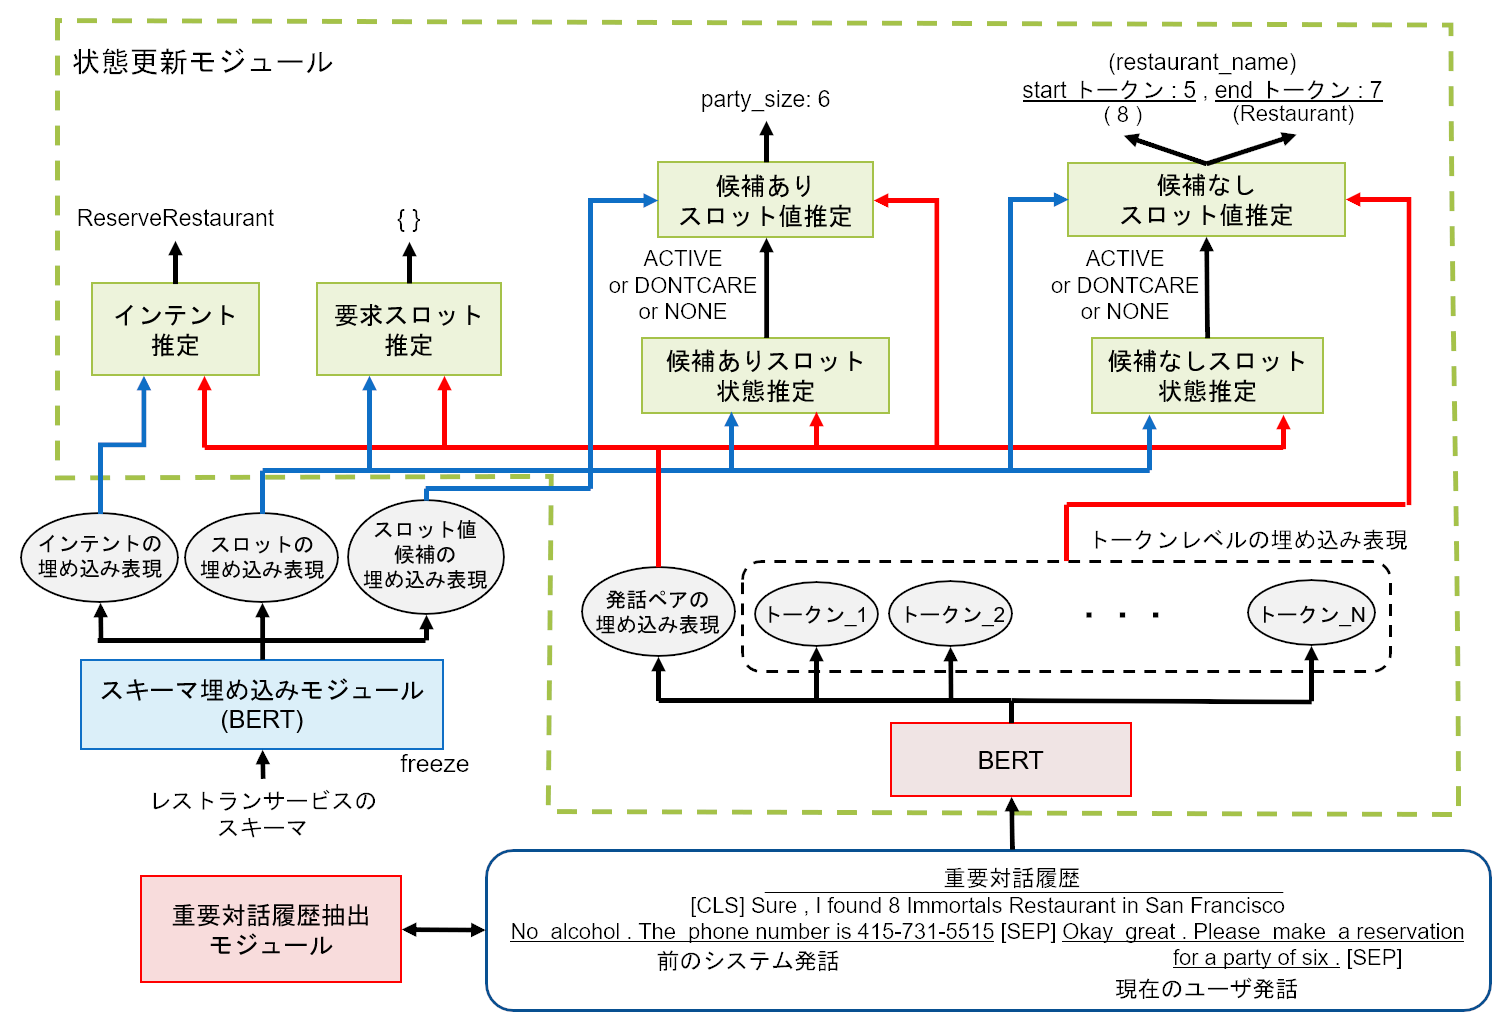
\includegraphics[width=15cm]{chapter4/teian2.eps}
  \caption{重要対話履歴抽出モジュールを加えた提案モデル}
  \label{fig:teianmodel}
\end{figure}

\begin{table}[thb]
  \centering
  \caption{SGDデータセットにある対話例の一部}
  \label{tab:taiwarei}
  \begin{tabularx}{\linewidth}{|p{55mm}|L|}\hline
    \multicolumn{1}{|c|}{
    \begin{tabular}{c}
      発話文\\(U:ユーザ,S:システム)
    \end{tabular}
    } 
    & \multicolumn{1}{|c|}{
      \begin{tabular}{c}
      対話状態(オレンジ色)or\\システムの対話行為(水色)
    \end{tabular}
     } \\ \hline \hline
     \rowcolor[rgb]{1.0,0.9,0.8}
    U1: Can you pull up a list of places to eat? & \{インテント:FindRestaurant, 要求スロット:[ ], スロット値:\{\} \}\\ \hline
    \rowcolor[rgb]{0.8, 1.0, 1.0}
    S1: Sure, what city should I search? And what kind of food would you like? & \{ REQUEST(city, [ ]), REQUEST(cuisine, [ ]) \} \\ \hline
    \rowcolor[rgb]{1.0,0.9,0.8}
    U2: Search San Francisco for Asian Fusion food & \{インテント:FindRestaurant, 要求スロット:[ ], スロット値:\{ city: San Fracisco, cuisine: Asian Fusion \} \} \\ \hline
    \rowcolor[rgb]{0.8, 1.0, 1.0}
    S2: Sure, I found 8 Immortals Restaurant in San Francisco & \{ OFFER(restaurant\_name, 8 Immortals Restaurant), OFFER(city, San Francisco) \} \\ \hline
    \rowcolor[rgb]{1.0,0.9,0.8}
    U3: Is there live music? & \{インテント:FindRestaurant, 要求スロット:[ has\_live\_music ], スロット値:\{ city: San Fracisco, cuisine: Asian Fusion \} \} \\ \hline
    \rowcolor[rgb]{0.8, 1.0, 1.0}
    S3: Unfortunately no. & \{ INFORM(has\_live\_music, False) \} \\ \hline
    \rowcolor[rgb]{1.0,0.9,0.8}
    U4: Do they serve alcohol? And what's their phone number? & \{インテント:FindRestaurant, 要求スロット:[ phone\_number, serves\_alcohol ], スロット値:\{ city: San Fracisco, cuisine: Asian Fusion \} \} \\ \hline
    \rowcolor[rgb]{0.8, 1.0, 1.0}
    S4: No alcohol. The phone number is 415-731-5515 & \{ INFORM(serves\_alocohol, False), INFORM(phone\_number, 415-731-5515) \} \\ \hline
    \rowcolor[rgb]{1.0,0.9,0.8}
    U5: Okay great. Please make a reservation for a party of six. & \{インテント:ReserveRestaurant, 要求スロット:[ ], スロット値:\{ city: San Fracisco, cuisine: Asian Fusion, party\_size: 6, restaurant\_name: 8 Immortals Restaurant \} \} \\ \hline
    \rowcolor[rgb]{0.8, 1.0, 1.0}
    \multicolumn{1}{|c|}{\vdots} & \multicolumn{1}{c|}{\vdots} \\ \hline
  \end{tabularx}
\end{table}

ベースラインモデルが過去の発話中に存在するスロット値を推定するために,対話履歴を用いる.深層学習による対話状態追跡で対話履歴を用いる場合,直近の数発話を履歴として入力に用いる\cite{trade,mrc}.しかし,直近の数発話では計算量の観点から多くの発話を入力するのは困難である.そこで,本研究では対話状態追跡に特に重要な発話をモデルへ入力するために,対話行為タグを用いた履歴抽出を提案する.この手法により,履歴として用いる発話を対話状態の推定に必要な情報を持つ発話のみにする.そのような発話を重要対話履歴とする.
\par

図\ref{fig:teianmodel}に示す提案モデルでは,ベースラインモデルの入力文を作成する箇所に重要対話履歴を抽出する重要対話履歴抽出モジュールを加えている.このモジュールは直前の最も重要度の高い履歴を1つ入力に加える.方法としては,入力文中にある前のターンのシステム発話が特定の対話行為タグを持つ場合にその発話を保持し,既に発話を保持している場合は新しい発話に更新する.そして,元々保持されていた発話を重要対話履歴として入力に加える.入力は,重要対話履歴,前のターンのシステム発話,現在のターンのユーザ発話の 3 発話となる.
\par
SGD データセットの対話例を表\ref{tab:taiwarei}に示す.表\ref{tab:taiwarei} では,n 回目のユーザ発話を Un,システム発話を Sn と表す.対話状態はユーザ発話が入力された後の状態を示していて,システムの対話行為はシステム発話に付与されているものを示している.この対話例では,S2 でシステムが提案したレストラン名に対して,U5 で了承してレストラン名が対話状態に反映される.この時,ユーザはレストラン名を過去の発話から暗黙的に参照しているため,発話中にレストラン名は含まれていない.そのため,S2 での発話を履歴として入力に加えて,レストラン名を示す “restaurant\_name” のスロット値となる “8 Immortals Restaurant” を推定可能にする必要がある.
\par
図 \ref{fig:teianmodel} では,例として表\ref{tab:taiwarei}のシステムの対話行為“OFFER”を持つ発話を抽出している.入力に加えられる重要対話履歴は,“8 Immortals Restaurant”を含む S2 での発話になる.入力文にスロット値となる文字列が含まれるため,スロット値として抜き出すことが可能になる.直近の数発話を対話履歴として用いる従来手法の場合は,直近の 6 発話を入力に加える必要があるが,提案手法では 3 発話で推定が行える.また,図\ref{fig:teianmodel}では5ターン前の発話を抽出しているが,提案手法はさらに前の発話を抽出することも可能である.ゆえに,提案手法は計算量の削減と同時に性能の向上が期待できる.
%-------------------------------------------------------------
\chapter{対話状態追跡における各対話行為の重要性調査}
\markright{対話状態追跡における各対話行為の重要性調査}
予備実験として,どの対話行為が対話状態追跡にとって重要なのかを調査する.本実験では,対話状態追跡においてスロット値を変更する候補を持つ発話が重要であると仮定する.ゆえに,対話行為ごとにスロット値候補の出現回数と出現したスロット値候補が実際にスロット値に反映された回数を調べて比較する.本章では,この2つの数値の調査方法の説明と調査結果を示す.
\section{データセット}
データセットはDSTC8-Track4 で公開された SGD データセット\cite{sgd}を用いる.対話データはユーザ役の対話シミュレータとシステム役の対話シミュレータによる対話を収集したものであり,各種ラベルもシミュレータによって付与されたものである.現在は学習用と検証用データのみ公開されている.SGD データセットは,対話中で1つのドメインしか扱わない Single-domain の対話と複数ドメインを扱う Multi-domain の対話という2種類を持つ.対話の長さは,Single-domainで平均$15.15$ターン,Multi-Domainで平均$22.94$ターンである.SGDデータセットは17個のドメインを扱う.そして,ドメインごとにサービスがいくつか存在し,スキーマが用意されている.ドメインごとのサービスの個数と,学習用,検証用データセットの対話数を表\ref{tab:taiwasu} に示す.また,SGDデータセットでは学習時,検証時,テスト時で扱うサービスが異なる.学習時と検証時で扱うサービスは表\ref{tab:service}に示す.スキーマに関しては付録の表\ref{tab:schema}に載せている.

\begin{table}[p]
    \begin{center}
    \begin{minipage}{1.0\hsize}
    \centering
    \caption{SGD データセットのドメインごとの対話数(括弧内はサービスの個数)}
    \label{tab:taiwasu}
    \vspace{3mm}
    \begin{tabular}{|l|c|c|c|c|c|c|} \hline
        & \multicolumn{3}{c|}{学習用の対話数} & \multicolumn{3}{|c|}{検証用の対話数}  \\ \cline{2-7}
        & \begin{tabular}{c}
            Single \\ domain
        \end{tabular} &
        \begin{tabular}{c}
            Multi \\ domain
        \end{tabular} & All 
        & \begin{tabular}{c}
            Single \\ domain
        \end{tabular} &
        \begin{tabular}{c}
            Multi \\ domain
        \end{tabular} & All \\ \hline
        Alarm (1) & NA & NA & NA & 37 & NA & 37  \\ \hline
        Banks (2) & 207 & 520 & 727  & 42 & 252 & 294  \\ \hline
        Buses (2) & 310 & 1,970 & 2,280  & 44 & 285 & 329  \\ \hline
        Calendar (1) & 169 & 1,433 & 1,602  & NA & NA & NA \\ \hline
        Events (2) & 788 & 2,721 & 3,509  & 73 & 345 & 418  \\ \hline
        Flights (3) & 985 & 1,762 & 2,747  & 94 & 297 & 391  \\ \hline
        Homes (1) & 268 & 579 & 847  & 81 & 99 & 180  \\ \hline
        Hotels (4) & 457 & 2,896 & 3,353  & 56 & 521 & 577  \\ \hline
        Media (2) & 281 & 832 & 1,113  & 46 & 133 & 179  \\ \hline
        Movies (2) & 292 & 1,325 & 1,617  & 47 & 94 & 141  \\ \hline
        Music (2) & 394 & 896 & 1,290  & 35 & 161 & 196  \\ \hline
        RentalCars (2) & 215 & 1,370 & 1,585  & 39 & 342 & 381  \\ \hline
        Restaurants (2) & 367 & 2052 & 2,419  & 73 & 263 & 336  \\ \hline
        RideSharing (2) & 119 & 1,584 & 1,703  & 45 & 225 & 270  \\ \hline
        Services (2) & 551 & 1,338 & 1,889  & 44 & 157 & 201  \\ \hline
        Travel (4) & NA & 1,871 & 1,871  & 45 & 238 & 283  \\ \hline
        Weather (1) & NA & 951 & 951  & 35 & 322 & 357  \\ \hline
        \textbf{TOTAL} & 5,403 & 10,739 & 16,142 & 836 & 1,646 & 2,482 \\ \hline
    \end{tabular}
    \end{minipage} \\

    \begin{minipage}{1.0\hsize}
    \centering
    \caption{SGD データセットの学習用,検証用が扱うサービスのリスト}
    \label{tab:service}
    \vspace{3mm}
    \begin{tabular}{|l|l|} \hline
        & \multicolumn{1}{c|}{扱うサービスのリスト} \\ \hline
        学習用 & 
        \begin{tabular}{l}
            [ Banks\_1, Buses\_1, Buses\_2, Calendar\_1, Events\_1, Events\_2, \\Flights\_1, Flights\_2, Homes\_1, Hotels\_1, Hotels\_2, Hotels\_3, Media\_1, \\Movies\_1, Music\_1, Music\_2, RentalCars\_1, RentalCars\_2, \\Restaurants\_1, RideSharing\_1, RideSharing\_2, Services\_1, Services\_2, \\Services\_3, Travel\_1, Weather\_1 ]
        \end{tabular} \\ \hline
        検証用 & 
        \begin{tabular}{l}
            [ Alarm\_1, Banks\_2, Buses\_1, Events\_1, Flights\_3, Homes\_1, Hotels\_1, \\Hotels\_4, Media\_2, Movies\_2, Music\_1, RentalCars\_1, Restaurants\_2, \\RideSharing\_1, Services\_4, Travel\_1, Weather\_1 ] 
        \end{tabular}\\ \hline
    \end{tabular}
    \end{minipage}
    \end{center}
\end{table}
\section{実験手法}
\begin{table}[htb]
    \centering
    \caption{SGDデータセットの学習用と検証用データにおける各対話行為の出現回数}
    \label{tab:action}
    \vspace{3mm}
    \begin{tabular}{|c|r|r|r|} \hline
        & \multicolumn{1}{c|}{Single-domain} & \multicolumn{1}{c|}{Multi-domain} & \multicolumn{1}{c|}{Combined} \\ \hline
        INFORM & 5,735 & 19,798 & 25,533 \\ \hline
        REQUEST & 9,772 & 29,841 & 39,613 \\ \hline
        CONFIRM & 6,417 & 18,213 & 24,630 \\ \hline
        OFFER & 10,276 & 33,887 & 44,163 \\ \hline
        NOTIFY\_SUCCESS & 4,215 & 12,254 & 16,469 \\ \hline
        NOTIFY\_FAILURE & 629 & 2,131 & 2,760 \\ \hline
        INFORM\_COUNT & 4,020 & 12,519 & 16,539 \\ \hline
        OFFER\_INTENT & 2,527 & 8,555 & 11,082 \\ \hline
        REQ\_MORE & 3,655 & 6,890 & 10,545 \\ \hline
        GOODBYE & 6,239 & 12,385 & 18,624 \\ \hline
        全システム発話 & 47,258 & 142,087 & 189,345 \\ \hline
    \end{tabular}
\end{table}

予備実験では SGD データセットの学習用と検証用のデータを全て使用した.対話数は18,624 対話,そのうちシステム発話は 189,345 発話ある.調査する発話は,対話行為タグが与えられるシステム発話に限定し,各発話の対話行為は発話が持つ対話行為タグで決定する.複数種類の対話行為タグを持つ場合は,対話行為も複数にしている.そのようにした場合の各対話行為の出現回数を表\ref{tab:action}に示す.このように各対話行為の出現回数には偏りがあるため,予備実験で示す結果は全て1対話あたりとする.なお,予備実験では,対話行為の“INFORM\_COUNT”と“OFFER\_INTENT”が与えるスロット値はスロット値の更新に関係ないため除外している.
\par
まず,各対話行為のスロット値候補の出現回数を調査した.スロット値候補は,各システム発話に与えられているスロット値範囲リストと対話行為リストを用いて重複を許さずに抽出される.各対話行為の発話からスロット値候補を抽出して,スロット値候補の出現回数をカウントしていく.全てをカウントしたのち,対話数で割ることで,1 対話あたりのスロット値候補の出現回数を各対話行為ごとに求める.

\par
続いて,各対話行為で出現したスロット値候補が実際にスロット値に反映された回数を調査した.まず,現在のターンの対話状態と前のターンの対話状態を比較して,現在のターンで追加されたスロット値を抽出する.そして現在のターンまでに各対話行為で出現したスロット値候補が何個含まれているかをカウントしていく.こちらも,スロット値候補の出現回数と同様に 1 対話あたりの数値を求める.
\section{調査結果}
\begin{figure}[thb]
    \begin{center}
        \begin{minipage}{1.0\hsize}
            \begin{center}
            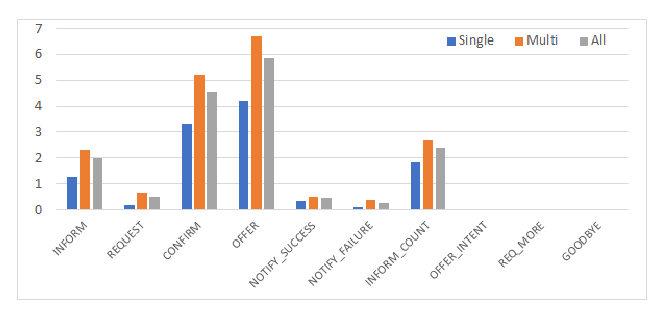
\includegraphics[clip, width=14cm]{chapter5/kouhoslot.eps}
            \caption{1対話あたりの各対話行為の発話中でスロット値候補が出現した回数}
            \label{fig:kouhoslot}
            \hspace{1.6cm}
            \end{center}
        \end{minipage}
        \begin{minipage}{1.0\hsize}
            \begin{center}
            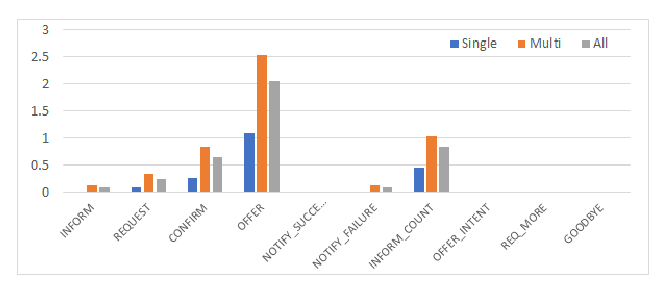
\includegraphics[clip, width=14cm]{chapter5/updateslot.eps}
            \caption{1対話あたりの各対話行為の発話中で出現したスロット値候補が実際にスロット値に反映された回数}
            \label{fig:updateslot}
            \end{center}
        \end{minipage}
    \end{center}
\end{figure}

結果は図\ref{fig:kouhoslot}と図\ref{fig:updateslot}に示す.この図では,Single-domain, Multi-domain,加えてその 2 つを合わせた All で結果に差異がないか調べるためにデータを分けて3つの結果を示している.図\ref{fig:kouhoslot}を見ると,“INFORM”と“CONFIRM”, “OFFER”, “INFORM\_COUNT”では他の対話行為に比べて多くのスロット値候補が出現していることが分かる.“INFORM”,“CONFIRM”,“OFFER”は,スロット値に関する発話を行うため,スロット値候補が多く出現している.ただし,“INFORM\_COUNT”はユーザの要求に合致する対象の個数を通知する対話行為であるため,それ自体がスロット値候補を与えることはないが,“OFFER”と同じ発話で共存していることが多い.そのため,“INFORM\_COUNT”の発話でもスロット値候補が多く出現している.残りの対話行為は,スロット値に関する発話を行わなず,他の対話行為と共存することも少ないため,発話中にスロット値候補が出現することが少ない.
\par
図\ref{fig:updateslot}を見ると,“INFORM”と“CONFIRM”は出現したスロット値候補に対して約10分の1しか対話状態に反映されていないことが分かる.これは両者ともに対話状態の更新に必要でないスロット値候補を多く与えているからである.例えば,“INFORM”が与えるスロット値候補はユーザが指定したものや場所の補足情報であり,対話状態を更新する情報ではないことが多い.また,“CONFIRM”の発話は既に対話状態に含まれているスロット値の確認を行うため,与えるスロット値候補の多くは既に対話状態に反映されており,対話状態が更新されない.ただし,“CONFIRM”が与えるスロット値候補は,ユーザが発した単語の言い換え(例:“at afternoon 1:30” $\rightarrow$ “1:30 pm”)を含むため対話状態にスロット値として追加されることもある.反対に,“OFFER”と“INFORM\_COUNT”は与えたスロット値候補の約4分の1が対話状態に反映されていることが分かる.したがって,両者どちらかの対話行為タグを持つ発話で出現するスロット値候補は対話状態に反映される可能性が高く,その発話は他の対話行為の発話よりスロット値の推定に重要であると考えられる.ただし,“CONFIRM”の説明で述べたように,対話行為ごとに与える情報に特徴があるため,一概に“OFFER”と“INFORM\_COUNT”を持つ発話だけが重要とは言えない.また,以上に示した結果は Single-domain, Multi-domain,加えてその 2 つを合わせた All でも同様の結果となっている.
%-------------------------------------------------------------
\chapter{評価実験}
本章では,実験条件を述べた上で提案手法を用いたモデルの性能について自動評価した結果を示す.その際,各対話行為タグで抽出した場合の性能比較,従来の対話履歴の使用法との性能比較を行う.自動評価の指標はDSTC8-Track4に従っている.
\markright{評価実験}
\section{実験条件}
モデルの実装には Tensorflow を用いている.実行環境は,産業技術総合研究所が構築し運用する,人工知能処理向け計算インフラストラクチャであるAI橋渡しクラウド(AI Bridging Cloud Infrastructure; ABCI)\cite{abci}を利用している.ABCIの計算資源はタイプ別に分かれているが,本研究では,CPU(Intel Xeon Gold 6148プロセッサー 2.4 GHz)が 5コア,GPU(NVIDIA Tesla V100 for NVLink 16GiB HBM2)が 1 個,メモリが 240 GiB,ローカルストレージが 180 GBの G.small を用いている.
\par
モデルの設定は,与えられたベースラインモデルとミニバッチサイズ以外全て同じにしている.BERT のハイパーパラメータはBERTの論文\cite{bert}に記載された $\verb|BERT|_{\verb|BASE|}$ の構成をそのまま使用する.つまり,BERTは隠れ層が 12 層,隠れ層のサイズが 768 次元である.学習はミニバッチ学習を行い,ミニバッチサイズを学習時は 32,検証時は 8,テスト時は 8 とする.ただし,従来の対話履歴の使用法との比較の際は,学習時のミニバッチサイズを 24 にして実験を行う.入力発話の最大長は,2発話入力の場合で 80 とし,1 発話増えるたびに 40 増加させる.学習率は 1e-4 とする.誤差関数には,交差エントロピーを使用し,最適化アルゴリズムは重み減衰によって過学習を抑制する Weight Decay という手法を用いた Adam \cite{adam} を使用する.過学習を防ぎモデルの汎化性能を上げるために,dropout(dropout 率は 0.1)を用いる.モデルは 80 epoch の学習を行い,学習を終えた段階のモデルを評価に使用する.
\par
データは Single-domain のみを用いて,学習用として 5,403 対話,検証用として 836 対話を学習に用いる.テスト用のデータはまだ未公開のため,今回は検証用データで評価している.

\section{評価指標}
モデルの自動評価は DSTC8-Track4 にて提供される自動評価スクリプトを用いた.そのスクリプトで計算される評価指標は 4 種類ある.1つ目はインテント推定の精度を示す Active Intent Accuracy,2つ目は要求スロット推定のマクロ平均 F1 スコアを示す Requested Slot F1,3つ目は各ターンでの対話状態の各スロット値の平均精度を示す Average Goal Accuracy,4つ目は各ターンでの対話状態の全スロット値の平均精度を示す Joint Goal Accuracy である.Requested Slot F1は,あるターンで予測結果と正解データどちらも要求スロットが存在しない場合そのターンをスキップするため,報告する数値はスキップされていない全てのユーザターンでの平均F1スコアとなる.Average Goal Accuracyは,正解データの対話状態で空でないスロットのみを対象としている.DSTC8-Track4 では Joint Goal Acuracy によってモデルの優劣をつけるため,本研究でも Joint Goal Accuracy の数値を重要視する.
\section{実験結果}
\begin{table}[thb]
    \centering
    \caption{各対話行為で提案手法を行った際の結果}
    \vspace{3mm}
    \label{tab:action_hikaku}
    \begin{tabular}{|c||r|r|r|r|} \hline
        &
        \begin{tabular}{c}
            Active \\ 
            Intent \\
            Accuracy
        \end{tabular} &
        \begin{tabular}{c}
            Requested \\
            Slot F1
        \end{tabular} &
        \begin{tabular}{c}
            Average \\ Goal \\ Accuracy
        \end{tabular} &
        \begin{tabular}{c}
            Joint \\ Goal \\ Accuracy
        \end{tabular}\\ \hline
        \begin{tabular}{c}
            ベースライン\\( 直近2発話入力 )
        \end{tabular} & 0.946 & 0.946 & 0.809 & 0.497 \\ \hline
        INFORM & 0.949 & 0.947 & 0.818 & 0.499 \\ \hline
        REQUEST & 0.946 & 0.946 & 0.807 & 0.495 \\ \hline
        CONFIRM & 0.960 & 0.946 & 0.807 & 0.497 \\ \hline
        OFFER & 0.957 & 0.945 & 0.851 & 0.572 \\ \hline
        NOTIFY\_SUCCESS & 0.956 & 0.948 & 0.813 & 0.500 \\ \hline
        NOTIFY\_FAILURE & 0.948 & 0.946 & 0.815 & 0.504 \\ \hline
        INFORM\_COUNT & 0.943 & 0.945 & 0.824 & 0.522 \\ \hline
        OFFER\_INTENT & 0.951 & 0.947 & 0.789 & 0.502 \\ \hline
        REQ\_MORE & 0.945 & 0.947 & 0.803 & 0.498 \\ \hline
        GOODBYE & 0.932 & 0.947 & 0.803 & 0.492 \\ \hline
    \end{tabular}
\end{table}
\begin{figure}[thb]
    \centering
    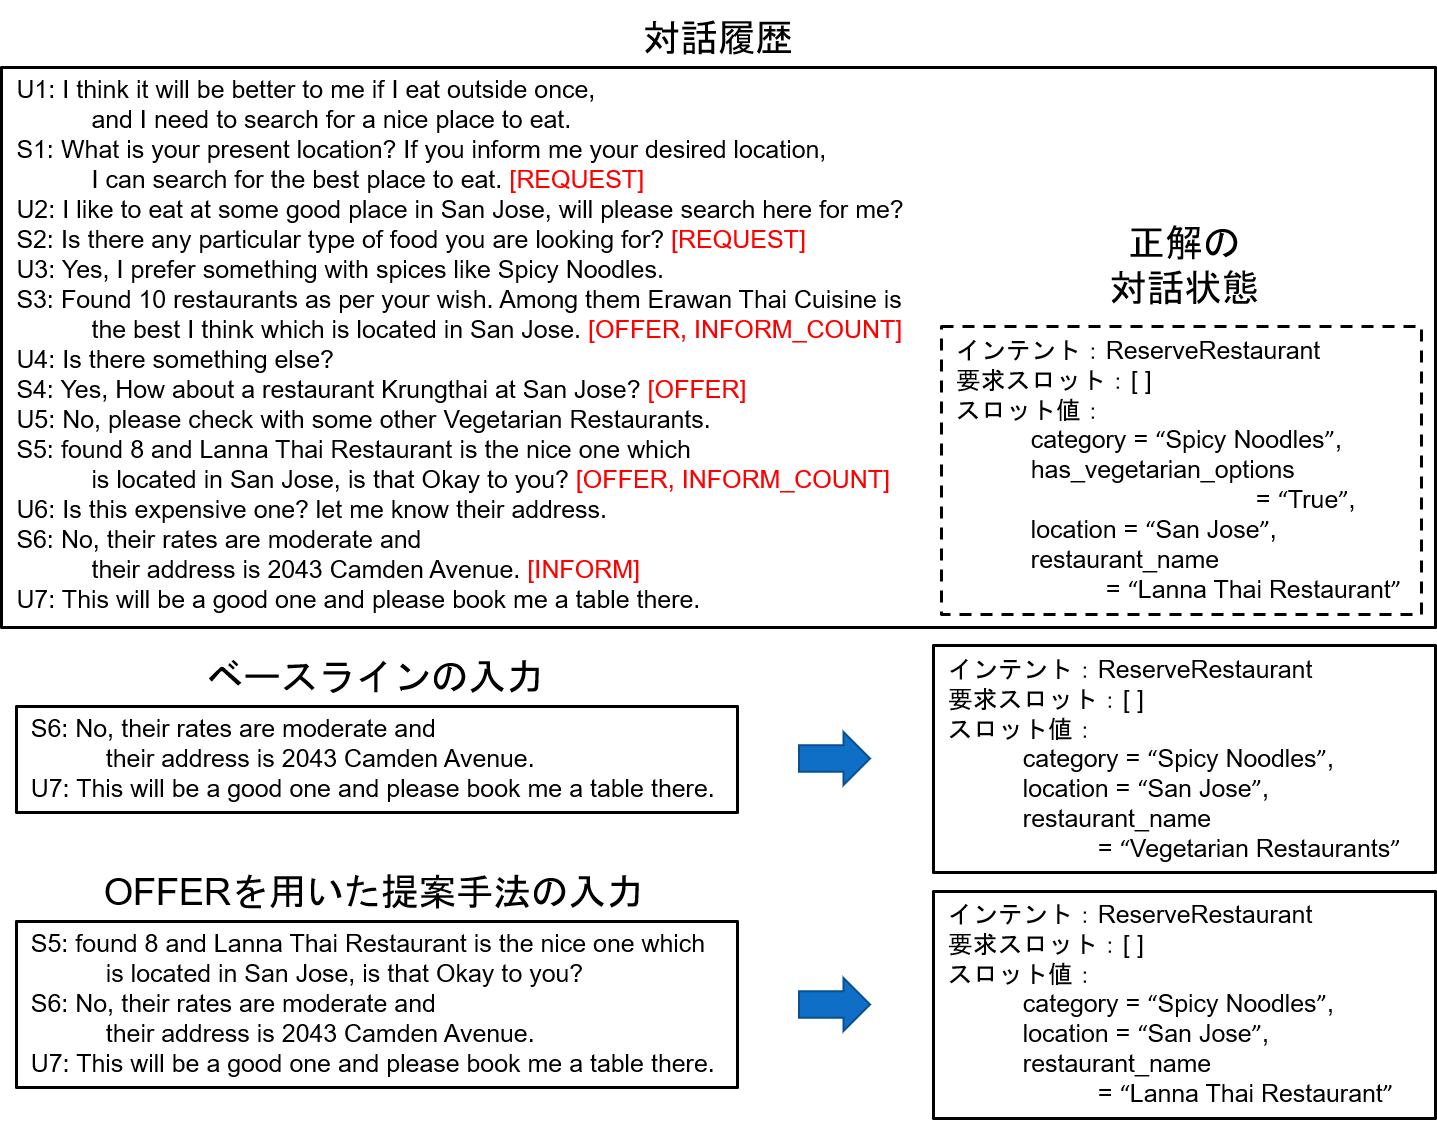
\includegraphics[width=15cm]{chapter6/case.eps}
    \caption{ベースラインとOFFERを用いた提案手法の出力結果}
    \label{fig:case}
\end{figure}

初めに,各対話行為タグを持つ発話がどの推定の性能を向上させるのかについて調べた.ベースラインモデルの結果と各対話行為タグで提案手法を行った際の結果を表\ref{tab:action_hikaku}に示す.Average Goal Accuracy をベースラインと比べると,“OFFER”が4.2\%, “INFORM\_COUNT”が 1.5\% 向上している.また,Joint Goal Accuracy をベースラインと比べると,“OFFER”が7.5\%, “INFORM\_COUNT”が 2.5\% 向上している.この結果は予備実験で示した通り,“OFFER” と “INFORM\_COUNT” を持つ発話が対話状態に反映されるスロット値候補を多く与えることと,図\ref{fig:case} に示したように過去の発話に存在するスロット値を推定可能になるからである.図\ref{fig:case} では“INFORM\_COUNT” でもレストラン名を推定できるが,“OFFER” と共存しない場合も存在するため,5.0\% の差が生まれている.他の対話行為の Average Goal Accuracy や Joint Goal Accuracy はベースラインと大差ないか減少しているため,スロット値推定に与える影響が少ない,もしくはその対話行為の発話がノイズとなっていると考えられる.また,図\ref{fig:case}では,候補ありスロットの“has\_vegetarian\_options”が推定できていない.このスロットは学習時に扱わない未知のスロットである.本研究では,未知のスロットや候補ありスロットに関しての対策を行っていないため,これらのスロット値推定の精度は向上していない.
\par

次に,Active Intent Accuracy をベースラインと比べると,“CONFIRM”が1.4\%, “OFFER”が1.1\%, “NOTIFY\_SUCCESS”が1.0\% 向上しているなど多くの対話行為で精度の向上が見られる.インテント推定はユーザの目的を推定しているので,対話の流れをより良く理解できる発話を履歴として入力できれば精度の向上が見込まれる.ゆえに,過去の発話を用いて情報量を増やした提案手法がベースラインの結果を超えている.ただし,対話の終わりに用いられる対話行為である“GOODBYE”は,対話の途中で抽出することはできないので精度が向上しなかった.また,インテント推定での誤りの多くは,最初の発話で異なるインテントを選択する誤りとインテントを維持すべきところで変更してしまう誤りであった.維持すべきところで変更してしまう誤りに関しては,前のターンのインテントをインテント推定の入力に用いることで解決すると期待できる.
\par
Requested Slot F1 に関しては大きな変化が見られない.つまり,要求スロットは現在のターンのユーザ発話の情報に大きく依存し,対話履歴では推定に必要な情報量があまり増加しない.
\par
ここまでの結果から,対話履歴をシステムの対話行為を用いて抽出することで性能が上がることを確認できた.今回は対話行為を 1 つだけ選択したが,複数の対話行為を用いることで更なる性能の向上が期待できる.

\begin{table}[thb]
    \centering
    \caption{従来手法との比較}
    \vspace{3mm}
    \label{tab:history_hikaku}
    \begin{tabular}{|c|r|r|r|r|r|} \hline
        &
        \begin{tabular}{c}
            Active \\ 
            Intent \\
            Accuracy
        \end{tabular} &
        \begin{tabular}{c}
            Requested \\
            Slot F1
        \end{tabular} &
        \begin{tabular}{c}
            Average \\ Goal \\ Accuracy
        \end{tabular} &
        \begin{tabular}{c}
            Joint \\ Goal \\ Accuracy
        \end{tabular} &
        \begin{tabular}{c}
            学習 \\ 時間
        \end{tabular} \\ \hline
        \begin{tabular}{c}
            ベースライン\\( 直近2発話\\入力 )
        \end{tabular} & 0.940 & 0.944 & 0.816 & 0.502 & 15.3(h)\\ \hline
        \begin{tabular}{c}
            提案手法 \\( OFFER )
        \end{tabular}
        & 0.946 & 0.947 & 0.845 & 0.565 & 20.7(h) \\ \hline
        直近3発話入力 & 0.943 & 0.947 & 0.815 & 0.508 & 20.9(h) \\ \hline
        直近4発話入力 & 0.974 & 0.948 & 0.844 & 0.553 & 26.3(h)\\ \hline
    \end{tabular}
\end{table}

続いて,従来の対話履歴の使用法との比較を行った.今回は提案手法として,他の対話行為より総合的に優れた結果を残した “OFFER” を用いた提案手法と,直近の2発話を入力としたモデル,3発話を入力としたモデル,4発話を入力としたモデルとを比較した.その結果を表\ref{tab:history_hikaku}に示す.ベースラインと提案手法の結果はミニバッチサイズを下げたことで変化している.直近3発話入力ではベースラインと比べて少ししか性能が向上していない.原因としては,1つ前のユーザ発話に含まれる既に推定済みの情報が現在のターンのユーザ発話に含まれる新しい情報の推定の妨げとなったことと,直近3発話では対話の流れを捉えるには情報不足であったことが考えられる.Joint Goal Accuracy に関しては,“OFFER”を用いた提案手法が直近3発話入力より5.7\% 高い数値を示している.同じ発話数でも性能が向上していることから,“OFFER”を用いた履歴抽出がスロット値推定に必要な情報を抽出できていることが分かる.また,提案手法は直近4発話入力よりJoint Goal Accuracyが1.2\% 高い数値を示している.これは,提案手法が対話によって6発話前や8発話前のスロット値も推定可能だからである.提案手法は3発話入力で直近4発話入力以上の結果を示していることから,対話状態追跡に重要な発話だけを抽出して重要ではない発話を取り除いているといえる.また,提案手法は直近4発話入力に比べて学習時間が5.4時間短く,計算量の削減にも成功している.しかし,Active Intent Accuracy では,直近4発話入力の方が提案手法に比べて 2.8\% 高い数値を示している.インテント推定は対話の流れを理解する必要があるため,連続した発話を入力する方が良い.そのため,提案手法のように過去の発話を抽出したものを用いると対話が断片的になり,連続した発話を入力とする従来手法より対話の流れを理解しにくいのだと考えられる.

%-------------------------------------------------------------
\chapter{むすび}                          % むすび
\markright{むすび}
本研究では,対話状態追跡における対話履歴の使い方として,対話行為タグを用いて重要な対話履歴を抽出する手法を提案した.DSTC8-Track4 で提供されたベースラインモデルと比較した結果,ユーザにスロット値候補を提案する “OFFER” という対話行為タグを用いたもので Joint Goal Accuracy が 7.5\% 向上した.直近の数発話を履歴として入力する従来手法と “OFFER” タグを用いた提案手法とを比較した結果,提案手法がモデルの学習時間を減らすのと同時に,性能を向上させることが可能であることを示した.
\par
今回の実験では“OFFER”を持つ発話のみを抽出した場合が最高の結果を示したが,他の対話行為と組み合わせて複数の対話行為を用いることで更なる性能の向上が期待できる.ゆえに,各対話行為タグが各ドメインにどのように影響するのかの調査を行い,対話行為タグの最適な組み合わせを見つけたい.
\par
今回の手法は人間が選択的にどの対話行為タグを持つ発話に注目するかを決めていた.この手法でも性能は向上するが,ドメインごとに注目すべき発話が異なる場合や他のデータセットの場合で重要な対話行為タグや対話履歴が変化するため対応ができない.そのため,機械側で対話履歴中のどの発話に注目すべきかを推定可能な対話状態追跡モデルを検討したい.


%-------------------------------------------------------------
\chapter*{謝辞}                           % 謝辞
\markright{謝辞}
\addcontentsline{toc}{chapter}{謝辞}
本研究を進めるにあたり,適切なご指導とご助言をいただきました李晃伸教授,酒向慎司准教授に深く感謝をいたします.また,共同で研究を行ってくださった李研究室博士前期課程 2 年田中涼太氏,尾関晃英氏,同研究室博士前期課程 1 年加藤修悟氏,研究環境の維持を含め,様々なご協力をいただいた同研究室博士前期課程 2 年森凜太朗氏をはじめ,李研究室の方々,また共に研究を進めた同期の方々に心より感謝をいたします.最後に,本学で研
究をする機会を与えてくださった両親と祖父母に感謝をいたします.


\newpage
%-------------------------------------------------------------
% 参考文献

\bibliography{biblio/bibtex}
\bibliographystyle{unsrt}


%-------------------------------------------------------------
% 付録
% 画像を沢山張り付ける場合など,

\chapter*{付録}
\markright{付録}
\addcontentsline{toc}{chapter}{付録}
\def\thechapter{A}
\section{各サービスのスキーマ}
\setlongtables
\begin{tabularx}{\linewidth}{|l|L|L|}
    \caption{各スキーマのスロットとインテント}
    \label{tab:schema}
    \\
    %------ 最初のページの表の最上部 ----
    \hline
    サービス & スロット & インテント \\ \hline
    \endfirsthead
    %------ 2ページ以降の表の最上部 ----
    \multicolumn{3}{l}{前ページからの続き} \\ \hline
    サービス & スロット & インテント \\ \hline
    \endhead
    %----- ページの表の最下部 --------
    \hline
    \multicolumn{3}{r}{表は次ページに続く}\\
    \endfoot
    %----- 最終ページの表の最下部 --------
    \hline
    \multicolumn{3}{r}{これで終了}\\
    \endlastfoot
    %----------------------------------------------------------------
    Alarm\_1 & [ 'alarm\_time', 'alarm\_name', 'new\_alarm\_time', 'new\_alarm\_name' ] & [ 'GetAlarms', 'AddAlarm' ] \\ \hline
    Banks\_1 & 
    [ 'account\_type', 'recipient\_account\_type', 'balance', 'amount', 'recipient\_account\_name' ] &
    [ 'CheckBalance', 'TransferMoney' ] \\ \hline 
    Banks\_2 & [ 'account\_type', 'recipient\_account\_type', 'account\_balance', 'transfer\_amount', 'recipient\_name', 'transfer\_time' ] & [ 'CheckBalance', 'TransferMoney' ] \\ \hline
    Buses\_1 & [ 'from\_location', 'to\_location', 'from\_station', 'to\_station', 'leaving\_date', 'leaving\_time', 'fare', 'travelers', 'transfers' ] & [ 'FindBus', 'BuyBusTicket' ] \\ \hline
    Buses\_2 & [ 'origin', 'destination', 'origin\_station\_name', 'destination\_station\_name', 'departure\_date', 'price', 'departure\_time', 'group\_size', 'fare\_type' ] & [ 'FindBus', 'BuyBusTicket' ] \\ \hline
    Calendar\_1 & [ 'event\_date', 'event\_time', 'event\_location', 'event\_name', 'available\_start\_time', 'available\_end\_time' ] & [ 'GetEvents', 'GetAvailableTime', 'AddEvent' ] \\ \hline
    Events\_1 & [ 'category', 'subcategory', 'event\_name', 'date', 'time', 'number\_of\_seats', 'city\_of\_event', 'event\_location', 'address\_of\_location' ] & [ 'FindEvents', 'BuyEventTickets' ] \\ \hline
    Events\_2 & [ 'event\_type', 'category', 'event\_name', 'date', 'time', 'number\_of\_tickets', 'city', 'venue', 'venue\_address' ] & [ 'FindEvents', 'GetEventDates', 'BuyEventTickets' ] \\ \hline
    Flights\_1 & [ 'passengers', 'seating\_class', 'origin\_city', 'destination\_city', 'origin\_airport', 'destination\_airport', 'departure\_date', 'return\_date', 'number\_stops', 'outbound\_departure\_time', 'outbound\_arrival\_time', 'inbound\_arrival\_time', 'inbound\_departure\_time', 'price', 'refundable', 'airlines' ] & [ 'SearchOnewayFlight', 'SearchRoundtripFlights', 'ReserveOnewayFlight', 'ReserveRoundtripFlights' ] \\ \hline
    Flights\_2 & [ 'passengers', 'seating\_class', 'origin', 'destination', 'origin\_airport', 'destination\_airport', 'departure\_date', 'return\_date', 'number\_stops', 'outbound\_departure\_time', 'outbound\_arrival\_time', 'inbound\_arrival\_time', 'inbound\_departure\_time', 'fare', 'is\_redeye', 'airlines' ] & [ 'SearchOnewayFlight', 'SearchRoundtripFlights' ] \\ \hline
    Flights\_3 & [ 'passengers', 'flight\_class', 'origin\_city', 'destination\_city', 'origin\_airport\_name', 'destination\_airport\_name', 'departure\_date', 'return\_date', 'number\_stops', 'outbound\_departure\_time', 'outbound\_arrival\_time', 'inbound\_arrival\_time', 'inbound\_departure\_time', 'price', 'number\_checked\_bags', 'airlines', 'arrives\_next\_day' ] & [ 'SearchOnewayFlight', 'SearchRoundtripFlights' ] \\ \hline
    Homes\_1 & [ 'area', 'address', 'property\_name', 'phone\_number', 'furnished', 'pets\_allowed', 'rent', 'visit\_date', 'number\_of\_beds', 'number\_of\_baths' ] & [ 'FindApartment', 'ScheduleVisit' ] \\ \hline
    Hotels\_1 & [ 'destination', 'number\_of\_rooms', 'check\_in\_date', 'number\_of\_days', 'star\_rating', 'hotel\_name', 'street\_address', 'phone\_number', 'price\_per\_night', 'has\_wifi' ] & [ 'ReserveHotel', 'SearchHotel' ] \\ \hline
    Hotels\_2 & [ 'where\_to', 'number\_of\_adults', 'check\_in\_date', 'check\_out\_date', 'rating', 'address', 'phone\_number', 'total\_price', 'has\_laundry\_service' ] & [ 'BookHouse', 'SearchHouse' ] \\ \hline
    Hotels\_3 & [ 'location', 'number\_of\_rooms', 'check\_in\_date', 'check\_out\_date', 'average\_rating', 'hotel\_name', 'street\_address', 'phone\_number', 'price', 'pets\_welcome' ] & [ 'ReserveHotel', 'SearchHotel' ] \\ \hline
    Hotels\_4 & [ 'location', 'number\_of\_rooms', 'check\_in\_date', 'stay\_length', 'star\_rating', 'place\_name', 'street\_address', 'phone\_number', 'price\_per\_night', 'smoking\_allowed' ] & [ 'ReserveHotel', 'SearchHotel' ] \\ \hline
    Media\_1 & [ 'title', 'genre', 'subtitles', 'directed\_by' ] & [ 'FindMovies', 'PlayMovie' ] \\ \hline
    Media\_2 & [ 'movie\_name', 'genre', 'subtitle\_language', 'director', 'actors', 'price' ] & [ 'FindMovies', 'RentMovie' ] \\ \hline
    Movies\_1 & [ 'price', 'number\_of\_tickets', 'show\_type', 'theater\_name', 'show\_time', 'show\_date', 'genre', 'street\_address', 'location', 'movie\_name' ] & [ 'BuyMovieTickets', 'FindMovies', 'GetTimesForMovie' ] \\ \hline
    Movies\_2 & [ 'title', 'genre', 'aggregate\_rating', 'starring', 'director' ] & [ 'FindMovies' ] \\ \hline
    Music\_1 & [ 'song\_name', 'artist', 'album', 'genre', 'year', 'playback\_device' ] & [ 'LookupSong', 'PlaySong' ] \\ \hline
    Music\_2 & [ 'song\_name', 'artist', 'album', 'genre', 'playback\_device' ] & [ 'LookupMusic', 'PlayMedia' ] \\ \hline
    RentalCars\_1 & [ 'type', 'car\_name', 'pickup\_location', 'pickup\_date', 'pickup\_time', 'pickup\_city', 'dropoff\_date', 'total\_price' ] & [ 'GetCarsAvailable', 'ReserveCar' ] \\ \hline
    RentalCars\_2 & [ 'car\_type', 'car\_name', 'pickup\_location', 'pickup\_date', 'pickup\_time', 'pickup\_city', 'dropoff\_date', 'total\_price' ] & [ 'GetCarsAvailable', 'ReserveCar' ] \\ \hline
    Restaurants\_1 & [ 'restaurant\_name', 'date', 'time', 'serves\_alcohol', 'has\_live\_music', 'phone\_number', 'street\_address', 'party\_size', 'price\_range', 'city', 'cuisine' ] & [ 'ReserveRestaurant', 'FindRestaurants' ] \\ \hline
    Restaurants\_2 & [ 'restaurant\_name', 'date', 'time', 'has\_seating\_outdoors', 'has\_vegetarian\_options', 'phone\_number', 'rating', 'address', 'number\_of\_seats', 'price\_range', 'location', 'category' ] & [ 'ReserveRestaurant', 'FindRestaurants' ] \\ \hline
    RideSharing\_1 & [ 'destination', 'shared\_ride', 'ride\_fare', 'approximate\_ride\_duration', 'number\_of\_riders' ] & [ 'GetRide' ] \\ \hline
    RideSharing\_2 & [ 'destination', 'ride\_type', 'ride\_fare', 'wait\_time', 'number\_of\_seats' ] & [ 'GetRide' ] \\ \hline
    Services\_1 & [ 'stylist\_name', 'phone\_number', 'average\_rating', 'is\_unisex', 'street\_address', 'city', 'appointment\_date', 'appointment\_time' ] & [ 'BookAppointment', 'FindProvider' ] \\ \hline
    Services\_2 & [ 'dentist\_name', 'phone\_number', 'address', 'city', 'appointment\_date', 'appointment\_time', 'offers\_cosmetic\_services' ] & [ 'BookAppointment', 'FindProvider' ] \\ \hline
    Services\_3 & [ 'doctor\_name', 'phone\_number', 'average\_rating', 'street\_address', 'city', 'appointment\_date', 'appointment\_time', 'type' ] & [ 'BookAppointment', 'FindProvider' ] \\ \hline
    Services\_4 & [ 'therapist\_name', 'phone\_number', 'address', 'city', 'appointment\_date', 'appointment\_time', 'type' ] & [ 'BookAppointment', 'FindProvider' ] \\ \hline
    Travel\_1 & [ 'location', 'attraction\_name', 'category', 'phone\_number', 'free\_entry', 'good\_for\_kids' ] & [ 'FindAttractions' ] \\ \hline
    Weather\_1 & [ 'precipitation', 'humidity', 'wind', 'temperature', 'city', 'date' ] & [ 'GetWeather' ] \\
\end{tabularx}

\end{document}
